\documentclass[twoside]{book}

% Packages required by doxygen
\usepackage{fixltx2e}
\usepackage{calc}
\usepackage{doxygen}
\usepackage[export]{adjustbox} % also loads graphicx
\usepackage{graphicx}
\usepackage[utf8]{inputenc}
\usepackage{makeidx}
\usepackage{multicol}
\usepackage{multirow}
\PassOptionsToPackage{warn}{textcomp}
\usepackage{textcomp}
\usepackage[nointegrals]{wasysym}
\usepackage[table]{xcolor}

% Font selection
\usepackage[T1]{fontenc}
\usepackage[scaled=.90]{helvet}
\usepackage{courier}
\usepackage{amssymb}
\usepackage{sectsty}
\renewcommand{\familydefault}{\sfdefault}
\allsectionsfont{%
  \fontseries{bc}\selectfont%
  \color{darkgray}%
}
\renewcommand{\DoxyLabelFont}{%
  \fontseries{bc}\selectfont%
  \color{darkgray}%
}
\newcommand{\+}{\discretionary{\mbox{\scriptsize$\hookleftarrow$}}{}{}}

% Page & text layout
\usepackage{geometry}
\geometry{%
  a4paper,%
  top=2.5cm,%
  bottom=2.5cm,%
  left=2.5cm,%
  right=2.5cm%
}
\tolerance=750
\hfuzz=15pt
\hbadness=750
\setlength{\emergencystretch}{15pt}
\setlength{\parindent}{0cm}
\setlength{\parskip}{3ex plus 2ex minus 2ex}
\makeatletter
\renewcommand{\paragraph}{%
  \@startsection{paragraph}{4}{0ex}{-1.0ex}{1.0ex}{%
    \normalfont\normalsize\bfseries\SS@parafont%
  }%
}
\renewcommand{\subparagraph}{%
  \@startsection{subparagraph}{5}{0ex}{-1.0ex}{1.0ex}{%
    \normalfont\normalsize\bfseries\SS@subparafont%
  }%
}
\makeatother

% Headers & footers
\usepackage{fancyhdr}
\pagestyle{fancyplain}
\fancyhead[LE]{\fancyplain{}{\bfseries\thepage}}
\fancyhead[CE]{\fancyplain{}{}}
\fancyhead[RE]{\fancyplain{}{\bfseries\leftmark}}
\fancyhead[LO]{\fancyplain{}{\bfseries\rightmark}}
\fancyhead[CO]{\fancyplain{}{}}
\fancyhead[RO]{\fancyplain{}{\bfseries\thepage}}
\fancyfoot[LE]{\fancyplain{}{}}
\fancyfoot[CE]{\fancyplain{}{}}
\fancyfoot[RE]{\fancyplain{}{\bfseries\scriptsize Generated by Doxygen }}
\fancyfoot[LO]{\fancyplain{}{\bfseries\scriptsize Generated by Doxygen }}
\fancyfoot[CO]{\fancyplain{}{}}
\fancyfoot[RO]{\fancyplain{}{}}
\renewcommand{\footrulewidth}{0.4pt}
\renewcommand{\chaptermark}[1]{%
  \markboth{#1}{}%
}
\renewcommand{\sectionmark}[1]{%
  \markright{\thesection\ #1}%
}

% Indices & bibliography
\usepackage{natbib}
\usepackage[titles]{tocloft}
\setcounter{tocdepth}{3}
\setcounter{secnumdepth}{5}
\makeindex

% Hyperlinks (required, but should be loaded last)
\usepackage{ifpdf}
\ifpdf
  \usepackage[pdftex,pagebackref=true]{hyperref}
\else
  \usepackage[ps2pdf,pagebackref=true]{hyperref}
\fi
\hypersetup{%
  colorlinks=true,%
  linkcolor=blue,%
  citecolor=blue,%
  unicode%
}

% Custom commands
\newcommand{\clearemptydoublepage}{%
  \newpage{\pagestyle{empty}\cleardoublepage}%
}

\usepackage{caption}
\captionsetup{labelsep=space,justification=centering,font={bf},singlelinecheck=off,skip=4pt,position=top}

%===== C O N T E N T S =====

\begin{document}

% Titlepage & ToC
\hypersetup{pageanchor=false,
             bookmarksnumbered=true,
             pdfencoding=unicode
            }
\pagenumbering{alph}
\begin{titlepage}
\vspace*{7cm}
\begin{center}%
{\Large My Project }\\
\vspace*{1cm}
{\large Generated by Doxygen 1.8.13}\\
\end{center}
\end{titlepage}
\clearemptydoublepage
\pagenumbering{roman}
\tableofcontents
\clearemptydoublepage
\pagenumbering{arabic}
\hypersetup{pageanchor=true}

%--- Begin generated contents ---
\chapter{Pink\+: A High Performance H\+T\+TP Server}
\label{md_README}
\Hypertarget{md_README}
{\bfseries Navigator}\+: {\bfseries https\+://github.com/\+Natureal/\+Pink\+\_\+server/blob/master/knowledge/architecture.\+md \char`\"{}架构与模块\char`\"{}} $\vert$$\vert$ {\bfseries https\+://github.com/\+Natureal/\+Pink\+\_\+server/blob/master/knowledge/evaluation.\+md \char`\"{}压力测试\char`\"{}} $\vert$$\vert$ {\bfseries https\+://github.com/\+Natureal/\+Pink\+\_\+server/blob/master/knowledge/problems.\+md \char`\"{}问题记录\char`\"{}} $\vert$$\vert$ {\bfseries https\+://github.com/\+Natureal/\+Pink\+\_\+server/blob/master/knowledge/basic.\+md \char`\"{}基础知识\char`\"{}}

{\bfseries Motivation}\+: 翻阅了书本以及学习了一些开源项目后,决定自己写一个 server,串联知识,探索一些小想法。 



\subsubsection*{Tools}


\begin{DoxyItemize}
\item {\bfseries 1. 开发环境}
\end{DoxyItemize}

(1) Ubuntu 18.\+04 (Linux Core 4.\+15)

(2) Intel i5-\/8250U (1.\+6(max\+: 3.\+4)G\+Hz $\ast$ 8)


\begin{DoxyItemize}
\item {\bfseries 2. 开发工具}
\end{DoxyItemize}

(1) Vim + Sublime Text 3 (C++11)

(2) C\+Make + ctags (源码定位器)


\begin{DoxyItemize}
\item {\bfseries 3. 测压工具}
\end{DoxyItemize}

(1) 单线程 I/O 复用方式\+: ./test/pressure\+\_\+test.cpp

(2) 多进程并发方法\+: {\bfseries \href{http://home.tiscali.cz/~cz210552/webbench.html}{\tt webbench}}

(3) 多线程 I/O 复用方式 (最高压力)\+: {\bfseries \href{https://github.com/wg/wrk}{\tt wrk}} 



\subsubsection*{Configuration}


\begin{DoxyItemize}
\item 端口号\+: 7777
\item 页面根目录\+: ./web
\item 连接池初始连接数\+: 2000(最大\+: 10\+K)
\item 线程池线程数量\+: 4
\item 非活动连接超时时间\+: 10s
\item 定期处理超时事件\+: 5s
\item Epoll 模式\+: et / lt 


\end{DoxyItemize}

\subsubsection*{To do list\+:}


\begin{DoxyEnumerate}
\item 实现自销毁的线程池(智能指针) {\bfseries Finished v1.\+0}
\item 添加定时器,实现自销毁的时间堆 {\bfseries Finished v1.\+0}
\item 优化定时器触发机制,学习内核 hrtimer
\item 实现自销毁的连接池 {\bfseries Finished v1.\+0}
\item 实现内存池(学习 S\+TL memory pool/tcmalloc/jemalloc)$\ast$$\ast$doing$\ast$$\ast$
\item 优化并行模式 -\/$>$ 优化的 Reactor 模式,省略一次性完成的写完成事件注册 {\bfseries Finished v1.\+0}
\item 生产者消费者,降低耦合 {\bfseries Finished v1.\+0}
\item 守护进程配置
\item 在线修改配置参数
\item 实现负载均衡(学习\+Ngin\+X)
\item 考虑https\+://github.com/\+Natureal/\+Pink\+\_\+server/blob/master/knowledge/E6\%83\%8AE7BEA4E9\%97AEE9A2\%98.\+md \char`\"{}线程池惊群问题\char`\"{} {\bfseries doing}
\item 探索 Proactor 模式\+: 完全异步 + 非阻塞模式 (A\+IO)
\item 考虑 pipeline 技术
\item 日志系统 
\end{DoxyEnumerate}
\chapter{Class Index}
\section{Class List}
Here are the classes, structs, unions and interfaces with brief descriptions\+:\begin{DoxyCompactList}
\item\contentsline{section}{\hyperlink{classcond}{cond} }{\pageref{classcond}}{}
\item\contentsline{section}{\hyperlink{structconfiguration}{configuration} }{\pageref{structconfiguration}}{}
\item\contentsline{section}{\hyperlink{classconn__timer}{conn\+\_\+timer} }{\pageref{classconn__timer}}{}
\item\contentsline{section}{\hyperlink{classmutex}{mutex} }{\pageref{classmutex}}{}
\item\contentsline{section}{\hyperlink{classpink__conn__pool}{pink\+\_\+conn\+\_\+pool$<$ T $>$} }{\pageref{classpink__conn__pool}}{}
\item\contentsline{section}{\hyperlink{classpink__http__conn}{pink\+\_\+http\+\_\+conn} }{\pageref{classpink__http__conn}}{}
\item\contentsline{section}{\hyperlink{classpink__http__machine}{pink\+\_\+http\+\_\+machine} }{\pageref{classpink__http__machine}}{}
\item\contentsline{section}{\hyperlink{classpink__threadpool}{pink\+\_\+threadpool$<$ T $>$} }{\pageref{classpink__threadpool}}{}
\item\contentsline{section}{\hyperlink{classpink__time__heap}{pink\+\_\+time\+\_\+heap} }{\pageref{classpink__time__heap}}{}
\item\contentsline{section}{\hyperlink{classsem}{sem} }{\pageref{classsem}}{}
\end{DoxyCompactList}

\chapter{Class Documentation}
\hypertarget{classconn__timer}{}\section{conn\+\_\+timer Class Reference}
\label{classconn__timer}\index{conn\+\_\+timer@{conn\+\_\+timer}}


{\ttfamily \#include $<$pink\+\_\+conn\+\_\+timer.\+h$>$}

\subsection*{Public Member Functions}
\begin{DoxyCompactItemize}
\item 
\hyperlink{classconn__timer_a0779436b23e1b67636349fb7c08cdf45}{conn\+\_\+timer} ()=default
\item 
\hyperlink{classconn__timer_a1f4ceab01f4274ab66147f4bb9fec535}{conn\+\_\+timer} (int delay, bool $\ast$init\+\_\+timeout)
\item 
void \hyperlink{classconn__timer_a543102358beb1bc590006310556182de}{cancel} ()
\item 
void \hyperlink{classconn__timer_a86d7a0d33b7423368bba281a0d0eaab9}{cb\+\_\+func} ()
\item 
void \hyperlink{classconn__timer_a6cb5ef510c4022acd31b002e15758d60}{reset} (int delay)
\end{DoxyCompactItemize}
\subsection*{Public Attributes}
\begin{DoxyCompactItemize}
\item 
time\+\_\+t \hyperlink{classconn__timer_a2c71b17e51d75dc27a4e0f1f7e443ec5}{expire}
\item 
bool \hyperlink{classconn__timer_a51dd2abd61d07bd63c37551404851bf5}{canceled}
\item 
bool $\ast$ \hyperlink{classconn__timer_a0f3fbb63bdf0764fffe4b5fd0fedc3db}{conn\+\_\+timeout}
\end{DoxyCompactItemize}


\subsection{Detailed Description}


Definition at line 7 of file pink\+\_\+conn\+\_\+timer.\+h.



\subsection{Constructor \& Destructor Documentation}
\mbox{\Hypertarget{classconn__timer_a0779436b23e1b67636349fb7c08cdf45}\label{classconn__timer_a0779436b23e1b67636349fb7c08cdf45}} 
\index{conn\+\_\+timer@{conn\+\_\+timer}!conn\+\_\+timer@{conn\+\_\+timer}}
\index{conn\+\_\+timer@{conn\+\_\+timer}!conn\+\_\+timer@{conn\+\_\+timer}}
\subsubsection{\texorpdfstring{conn\+\_\+timer()}{conn\_timer()}\hspace{0.1cm}{\footnotesize\ttfamily [1/2]}}
{\footnotesize\ttfamily conn\+\_\+timer\+::conn\+\_\+timer (\begin{DoxyParamCaption}{ }\end{DoxyParamCaption})\hspace{0.3cm}{\ttfamily [default]}}

\mbox{\Hypertarget{classconn__timer_a1f4ceab01f4274ab66147f4bb9fec535}\label{classconn__timer_a1f4ceab01f4274ab66147f4bb9fec535}} 
\index{conn\+\_\+timer@{conn\+\_\+timer}!conn\+\_\+timer@{conn\+\_\+timer}}
\index{conn\+\_\+timer@{conn\+\_\+timer}!conn\+\_\+timer@{conn\+\_\+timer}}
\subsubsection{\texorpdfstring{conn\+\_\+timer()}{conn\_timer()}\hspace{0.1cm}{\footnotesize\ttfamily [2/2]}}
{\footnotesize\ttfamily conn\+\_\+timer\+::conn\+\_\+timer (\begin{DoxyParamCaption}\item[{int}]{delay,  }\item[{bool $\ast$}]{init\+\_\+timeout }\end{DoxyParamCaption})\hspace{0.3cm}{\ttfamily [inline]}}



Definition at line 10 of file pink\+\_\+conn\+\_\+timer.\+h.



\subsection{Member Function Documentation}
\mbox{\Hypertarget{classconn__timer_a543102358beb1bc590006310556182de}\label{classconn__timer_a543102358beb1bc590006310556182de}} 
\index{conn\+\_\+timer@{conn\+\_\+timer}!cancel@{cancel}}
\index{cancel@{cancel}!conn\+\_\+timer@{conn\+\_\+timer}}
\subsubsection{\texorpdfstring{cancel()}{cancel()}}
{\footnotesize\ttfamily void conn\+\_\+timer\+::cancel (\begin{DoxyParamCaption}{ }\end{DoxyParamCaption})\hspace{0.3cm}{\ttfamily [inline]}}



Definition at line 15 of file pink\+\_\+conn\+\_\+timer.\+h.

Here is the caller graph for this function\+:
\nopagebreak
\begin{figure}[H]
\begin{center}
\leavevmode
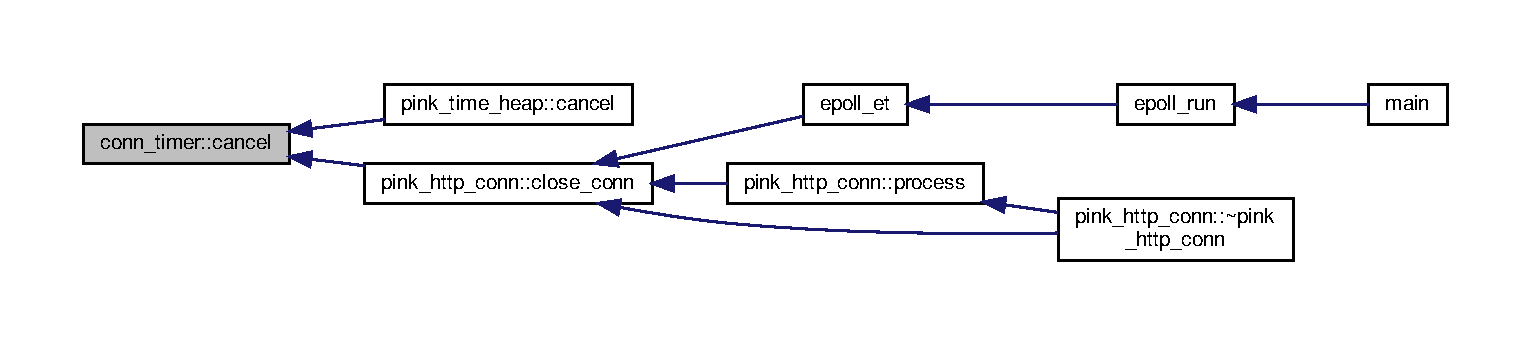
\includegraphics[width=350pt]{classconn__timer_a543102358beb1bc590006310556182de_icgraph}
\end{center}
\end{figure}
\mbox{\Hypertarget{classconn__timer_a86d7a0d33b7423368bba281a0d0eaab9}\label{classconn__timer_a86d7a0d33b7423368bba281a0d0eaab9}} 
\index{conn\+\_\+timer@{conn\+\_\+timer}!cb\+\_\+func@{cb\+\_\+func}}
\index{cb\+\_\+func@{cb\+\_\+func}!conn\+\_\+timer@{conn\+\_\+timer}}
\subsubsection{\texorpdfstring{cb\+\_\+func()}{cb\_func()}}
{\footnotesize\ttfamily void conn\+\_\+timer\+::cb\+\_\+func (\begin{DoxyParamCaption}{ }\end{DoxyParamCaption})\hspace{0.3cm}{\ttfamily [inline]}}



Definition at line 16 of file pink\+\_\+conn\+\_\+timer.\+h.

Here is the caller graph for this function\+:
\nopagebreak
\begin{figure}[H]
\begin{center}
\leavevmode
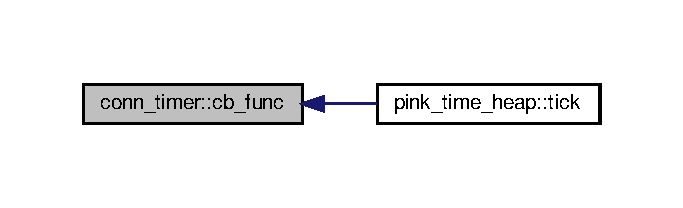
\includegraphics[width=328pt]{classconn__timer_a86d7a0d33b7423368bba281a0d0eaab9_icgraph}
\end{center}
\end{figure}
\mbox{\Hypertarget{classconn__timer_a6cb5ef510c4022acd31b002e15758d60}\label{classconn__timer_a6cb5ef510c4022acd31b002e15758d60}} 
\index{conn\+\_\+timer@{conn\+\_\+timer}!reset@{reset}}
\index{reset@{reset}!conn\+\_\+timer@{conn\+\_\+timer}}
\subsubsection{\texorpdfstring{reset()}{reset()}}
{\footnotesize\ttfamily void conn\+\_\+timer\+::reset (\begin{DoxyParamCaption}\item[{int}]{delay }\end{DoxyParamCaption})\hspace{0.3cm}{\ttfamily [inline]}}



Definition at line 17 of file pink\+\_\+conn\+\_\+timer.\+h.

Here is the caller graph for this function\+:
\nopagebreak
\begin{figure}[H]
\begin{center}
\leavevmode
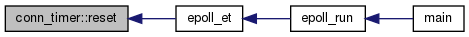
\includegraphics[width=350pt]{classconn__timer_a6cb5ef510c4022acd31b002e15758d60_icgraph}
\end{center}
\end{figure}


\subsection{Member Data Documentation}
\mbox{\Hypertarget{classconn__timer_a51dd2abd61d07bd63c37551404851bf5}\label{classconn__timer_a51dd2abd61d07bd63c37551404851bf5}} 
\index{conn\+\_\+timer@{conn\+\_\+timer}!canceled@{canceled}}
\index{canceled@{canceled}!conn\+\_\+timer@{conn\+\_\+timer}}
\subsubsection{\texorpdfstring{canceled}{canceled}}
{\footnotesize\ttfamily bool conn\+\_\+timer\+::canceled}



Definition at line 23 of file pink\+\_\+conn\+\_\+timer.\+h.

\mbox{\Hypertarget{classconn__timer_a0f3fbb63bdf0764fffe4b5fd0fedc3db}\label{classconn__timer_a0f3fbb63bdf0764fffe4b5fd0fedc3db}} 
\index{conn\+\_\+timer@{conn\+\_\+timer}!conn\+\_\+timeout@{conn\+\_\+timeout}}
\index{conn\+\_\+timeout@{conn\+\_\+timeout}!conn\+\_\+timer@{conn\+\_\+timer}}
\subsubsection{\texorpdfstring{conn\+\_\+timeout}{conn\_timeout}}
{\footnotesize\ttfamily bool$\ast$ conn\+\_\+timer\+::conn\+\_\+timeout}



Definition at line 24 of file pink\+\_\+conn\+\_\+timer.\+h.

\mbox{\Hypertarget{classconn__timer_a2c71b17e51d75dc27a4e0f1f7e443ec5}\label{classconn__timer_a2c71b17e51d75dc27a4e0f1f7e443ec5}} 
\index{conn\+\_\+timer@{conn\+\_\+timer}!expire@{expire}}
\index{expire@{expire}!conn\+\_\+timer@{conn\+\_\+timer}}
\subsubsection{\texorpdfstring{expire}{expire}}
{\footnotesize\ttfamily time\+\_\+t conn\+\_\+timer\+::expire}



Definition at line 22 of file pink\+\_\+conn\+\_\+timer.\+h.



The documentation for this class was generated from the following file\+:\begin{DoxyCompactItemize}
\item 
\hyperlink{pink__conn__timer_8h}{pink\+\_\+conn\+\_\+timer.\+h}\end{DoxyCompactItemize}

\hypertarget{classpink__conn__pool}{}\section{pink\+\_\+conn\+\_\+pool$<$ T $>$ Class Template Reference}
\label{classpink__conn__pool}\index{pink\+\_\+conn\+\_\+pool$<$ T $>$@{pink\+\_\+conn\+\_\+pool$<$ T $>$}}
\subsection*{Public Member Functions}
\begin{DoxyCompactItemize}
\item 
\mbox{\Hypertarget{classpink__conn__pool_a5c557c48815d595f7897f6abc8e55758}\label{classpink__conn__pool_a5c557c48815d595f7897f6abc8e55758}} 
{\bfseries pink\+\_\+conn\+\_\+pool} (int init\+\_\+cur\+\_\+number, int init\+\_\+max\+\_\+number)
\item 
\mbox{\Hypertarget{classpink__conn__pool_a1b053641006c7f00fd4764fea40f410c}\label{classpink__conn__pool_a1b053641006c7f00fd4764fea40f410c}} 
T $\ast$ {\bfseries get\+\_\+conn} ()
\item 
\mbox{\Hypertarget{classpink__conn__pool_a331df25708f142559d051ab8859ed707}\label{classpink__conn__pool_a331df25708f142559d051ab8859ed707}} 
void {\bfseries return\+\_\+conn} (T $\ast$conn)
\item 
\mbox{\Hypertarget{classpink__conn__pool_a90965493d13fc28f0060ca6fed7d12a4}\label{classpink__conn__pool_a90965493d13fc28f0060ca6fed7d12a4}} 
int {\bfseries get\+\_\+used\+\_\+number} ()
\end{DoxyCompactItemize}


The documentation for this class was generated from the following file\+:\begin{DoxyCompactItemize}
\item 
pink\+\_\+conn\+\_\+pool.\+h\end{DoxyCompactItemize}

\hypertarget{classpink__http__conn}{}\section{pink\+\_\+http\+\_\+conn Class Reference}
\label{classpink__http__conn}\index{pink\+\_\+http\+\_\+conn@{pink\+\_\+http\+\_\+conn}}


{\ttfamily \#include $<$pink\+\_\+http\+\_\+conn.\+h$>$}



Collaboration diagram for pink\+\_\+http\+\_\+conn\+:\nopagebreak
\begin{figure}[H]
\begin{center}
\leavevmode
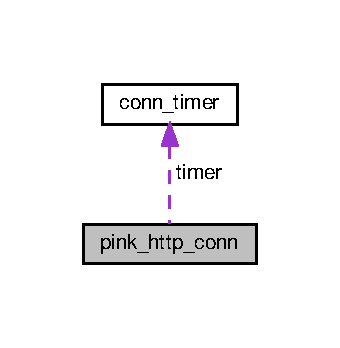
\includegraphics[width=163pt]{classpink__http__conn__coll__graph}
\end{center}
\end{figure}
\subsection*{Public Types}
\begin{DoxyCompactItemize}
\item 
enum \hyperlink{classpink__http__conn_a7959fd18f89efd188dcbc662ff65ddcb}{O\+P\+\_\+\+T\+Y\+PE} \{ \hyperlink{classpink__http__conn_a7959fd18f89efd188dcbc662ff65ddcba811e1ebb2bb8557c98390936e96af25e}{R\+E\+AD} = 0, 
\hyperlink{classpink__http__conn_a7959fd18f89efd188dcbc662ff65ddcba36bef4cc85522d8b97cabc2a031d5dfd}{W\+R\+I\+TE}
 \}
\end{DoxyCompactItemize}
\subsection*{Public Member Functions}
\begin{DoxyCompactItemize}
\item 
\hyperlink{classpink__http__conn_afd3fc76ed1b043d5041741081a2c38ee}{pink\+\_\+http\+\_\+conn} ()
\item 
\hyperlink{classpink__http__conn_a83eb4a1a4b8afdc6bfa0959da37f0e91}{$\sim$pink\+\_\+http\+\_\+conn} ()
\item 
void \hyperlink{classpink__http__conn_abff27697496d209cdc7375f99117f018}{init} (int sockfd, const sockaddr\+\_\+in \&addr)
\item 
void \hyperlink{classpink__http__conn_a14ed30d2643f52ec95c45b11b13b2411}{init\+\_\+listen} (int sockfd)
\item 
void \hyperlink{classpink__http__conn_abdcd7c0da8072d62cb7212523f20298b}{close\+\_\+conn} ()
\item 
void \hyperlink{classpink__http__conn_a41ca12d76d0056562633f27d456d0b62}{process} (int flag)
\item 
bool \hyperlink{classpink__http__conn_a254c09e8b962e5a0bc116f8da271b5ed}{read} ()
\item 
bool \hyperlink{classpink__http__conn_a362df085394bbf2818c8af93932c80d5}{write} ()
\item 
int \hyperlink{classpink__http__conn_aa304899ec9a7f6d7a2a9d738309a9570}{get\+\_\+fd} ()
\end{DoxyCompactItemize}
\subsection*{Public Attributes}
\begin{DoxyCompactItemize}
\item 
\hyperlink{classconn__timer}{conn\+\_\+timer} $\ast$ \hyperlink{classpink__http__conn_a0b34c6a8a6b8f65fa882adb109990e43}{timer}
\item 
bool \hyperlink{classpink__http__conn_a8687eb679249e4ae085c319dd2d4dfc7}{timeout}
\end{DoxyCompactItemize}
\subsection*{Static Public Attributes}
\begin{DoxyCompactItemize}
\item 
static void($\ast$ \hyperlink{classpink__http__conn_a36a48a19aa593001494eb51106628ebd}{delete\+\_\+cb\+\_\+func} )(\hyperlink{classpink__http__conn}{pink\+\_\+http\+\_\+conn} $\ast$conn) = nullptr
\item 
static const int \hyperlink{classpink__http__conn_a240ddaa8b2707d66601b1b82c002ef96}{R\+E\+A\+D\+\_\+\+B\+U\+F\+F\+E\+R\+\_\+\+S\+I\+ZE} = 2048
\item 
static const int \hyperlink{classpink__http__conn_a7764e0564be1e1ae66c44cf34550efea}{W\+R\+I\+T\+E\+\_\+\+B\+U\+F\+F\+E\+R\+\_\+\+S\+I\+ZE} = 1024
\item 
static int \hyperlink{classpink__http__conn_a106c011c818e2a80dbb14c61abbe9a2a}{epollfd} = -\/1
\item 
static int \hyperlink{classpink__http__conn_a4796952e9f7dc2a940e5681bc8f04139}{user\+\_\+count} = 0
\end{DoxyCompactItemize}


\subsection{Detailed Description}


Definition at line 15 of file pink\+\_\+http\+\_\+conn.\+h.



\subsection{Member Enumeration Documentation}
\mbox{\Hypertarget{classpink__http__conn_a7959fd18f89efd188dcbc662ff65ddcb}\label{classpink__http__conn_a7959fd18f89efd188dcbc662ff65ddcb}} 
\index{pink\+\_\+http\+\_\+conn@{pink\+\_\+http\+\_\+conn}!O\+P\+\_\+\+T\+Y\+PE@{O\+P\+\_\+\+T\+Y\+PE}}
\index{O\+P\+\_\+\+T\+Y\+PE@{O\+P\+\_\+\+T\+Y\+PE}!pink\+\_\+http\+\_\+conn@{pink\+\_\+http\+\_\+conn}}
\subsubsection{\texorpdfstring{O\+P\+\_\+\+T\+Y\+PE}{OP\_TYPE}}
{\footnotesize\ttfamily enum \hyperlink{classpink__http__conn_a7959fd18f89efd188dcbc662ff65ddcb}{pink\+\_\+http\+\_\+conn\+::\+O\+P\+\_\+\+T\+Y\+PE}}

\begin{DoxyEnumFields}{Enumerator}
\raisebox{\heightof{T}}[0pt][0pt]{\index{R\+E\+AD@{R\+E\+AD}!pink\+\_\+http\+\_\+conn@{pink\+\_\+http\+\_\+conn}}\index{pink\+\_\+http\+\_\+conn@{pink\+\_\+http\+\_\+conn}!R\+E\+AD@{R\+E\+AD}}}\mbox{\Hypertarget{classpink__http__conn_a7959fd18f89efd188dcbc662ff65ddcba811e1ebb2bb8557c98390936e96af25e}\label{classpink__http__conn_a7959fd18f89efd188dcbc662ff65ddcba811e1ebb2bb8557c98390936e96af25e}} 
R\+E\+AD&\\
\hline

\raisebox{\heightof{T}}[0pt][0pt]{\index{W\+R\+I\+TE@{W\+R\+I\+TE}!pink\+\_\+http\+\_\+conn@{pink\+\_\+http\+\_\+conn}}\index{pink\+\_\+http\+\_\+conn@{pink\+\_\+http\+\_\+conn}!W\+R\+I\+TE@{W\+R\+I\+TE}}}\mbox{\Hypertarget{classpink__http__conn_a7959fd18f89efd188dcbc662ff65ddcba36bef4cc85522d8b97cabc2a031d5dfd}\label{classpink__http__conn_a7959fd18f89efd188dcbc662ff65ddcba36bef4cc85522d8b97cabc2a031d5dfd}} 
W\+R\+I\+TE&\\
\hline

\end{DoxyEnumFields}


Definition at line 35 of file pink\+\_\+http\+\_\+conn.\+h.



\subsection{Constructor \& Destructor Documentation}
\mbox{\Hypertarget{classpink__http__conn_afd3fc76ed1b043d5041741081a2c38ee}\label{classpink__http__conn_afd3fc76ed1b043d5041741081a2c38ee}} 
\index{pink\+\_\+http\+\_\+conn@{pink\+\_\+http\+\_\+conn}!pink\+\_\+http\+\_\+conn@{pink\+\_\+http\+\_\+conn}}
\index{pink\+\_\+http\+\_\+conn@{pink\+\_\+http\+\_\+conn}!pink\+\_\+http\+\_\+conn@{pink\+\_\+http\+\_\+conn}}
\subsubsection{\texorpdfstring{pink\+\_\+http\+\_\+conn()}{pink\_http\_conn()}}
{\footnotesize\ttfamily pink\+\_\+http\+\_\+conn\+::pink\+\_\+http\+\_\+conn (\begin{DoxyParamCaption}{ }\end{DoxyParamCaption})\hspace{0.3cm}{\ttfamily [inline]}}



Definition at line 17 of file pink\+\_\+http\+\_\+conn.\+h.

\mbox{\Hypertarget{classpink__http__conn_a83eb4a1a4b8afdc6bfa0959da37f0e91}\label{classpink__http__conn_a83eb4a1a4b8afdc6bfa0959da37f0e91}} 
\index{pink\+\_\+http\+\_\+conn@{pink\+\_\+http\+\_\+conn}!````~pink\+\_\+http\+\_\+conn@{$\sim$pink\+\_\+http\+\_\+conn}}
\index{````~pink\+\_\+http\+\_\+conn@{$\sim$pink\+\_\+http\+\_\+conn}!pink\+\_\+http\+\_\+conn@{pink\+\_\+http\+\_\+conn}}
\subsubsection{\texorpdfstring{$\sim$pink\+\_\+http\+\_\+conn()}{~pink\_http\_conn()}}
{\footnotesize\ttfamily pink\+\_\+http\+\_\+conn\+::$\sim$pink\+\_\+http\+\_\+conn (\begin{DoxyParamCaption}{ }\end{DoxyParamCaption})\hspace{0.3cm}{\ttfamily [inline]}}



Definition at line 18 of file pink\+\_\+http\+\_\+conn.\+h.

Here is the call graph for this function\+:\nopagebreak
\begin{figure}[H]
\begin{center}
\leavevmode
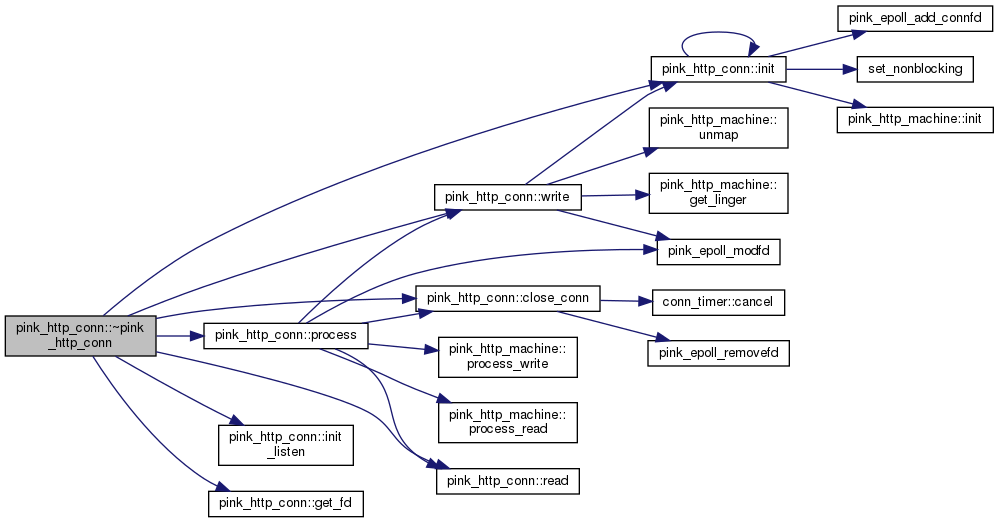
\includegraphics[width=350pt]{classpink__http__conn_a83eb4a1a4b8afdc6bfa0959da37f0e91_cgraph}
\end{center}
\end{figure}


\subsection{Member Function Documentation}
\mbox{\Hypertarget{classpink__http__conn_abdcd7c0da8072d62cb7212523f20298b}\label{classpink__http__conn_abdcd7c0da8072d62cb7212523f20298b}} 
\index{pink\+\_\+http\+\_\+conn@{pink\+\_\+http\+\_\+conn}!close\+\_\+conn@{close\+\_\+conn}}
\index{close\+\_\+conn@{close\+\_\+conn}!pink\+\_\+http\+\_\+conn@{pink\+\_\+http\+\_\+conn}}
\subsubsection{\texorpdfstring{close\+\_\+conn()}{close\_conn()}}
{\footnotesize\ttfamily void pink\+\_\+http\+\_\+conn\+::close\+\_\+conn (\begin{DoxyParamCaption}{ }\end{DoxyParamCaption})}



Definition at line 11 of file pink\+\_\+http\+\_\+conn.\+cpp.

Here is the call graph for this function\+:\nopagebreak
\begin{figure}[H]
\begin{center}
\leavevmode
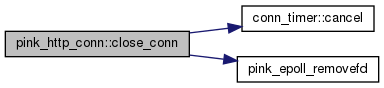
\includegraphics[width=350pt]{classpink__http__conn_abdcd7c0da8072d62cb7212523f20298b_cgraph}
\end{center}
\end{figure}
Here is the caller graph for this function\+:
\nopagebreak
\begin{figure}[H]
\begin{center}
\leavevmode
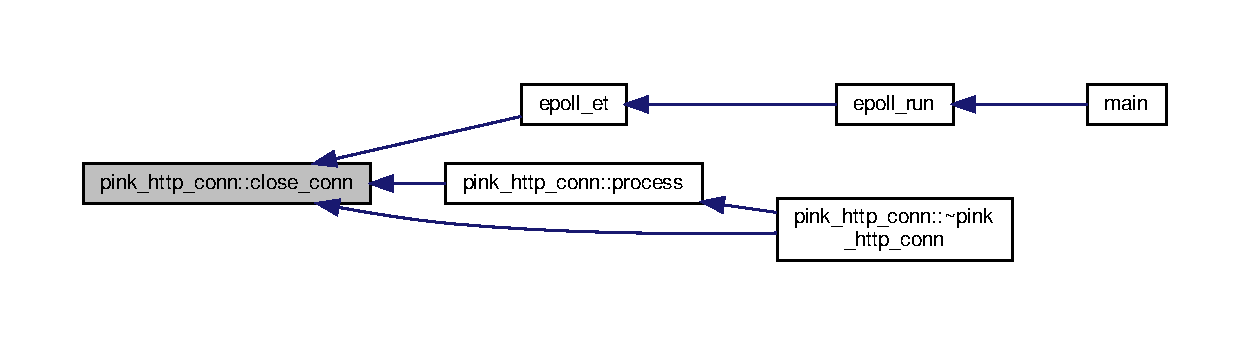
\includegraphics[width=350pt]{classpink__http__conn_abdcd7c0da8072d62cb7212523f20298b_icgraph}
\end{center}
\end{figure}
\mbox{\Hypertarget{classpink__http__conn_aa304899ec9a7f6d7a2a9d738309a9570}\label{classpink__http__conn_aa304899ec9a7f6d7a2a9d738309a9570}} 
\index{pink\+\_\+http\+\_\+conn@{pink\+\_\+http\+\_\+conn}!get\+\_\+fd@{get\+\_\+fd}}
\index{get\+\_\+fd@{get\+\_\+fd}!pink\+\_\+http\+\_\+conn@{pink\+\_\+http\+\_\+conn}}
\subsubsection{\texorpdfstring{get\+\_\+fd()}{get\_fd()}}
{\footnotesize\ttfamily int pink\+\_\+http\+\_\+conn\+::get\+\_\+fd (\begin{DoxyParamCaption}{ }\end{DoxyParamCaption})}



Definition at line 7 of file pink\+\_\+http\+\_\+conn.\+cpp.

Here is the caller graph for this function\+:
\nopagebreak
\begin{figure}[H]
\begin{center}
\leavevmode
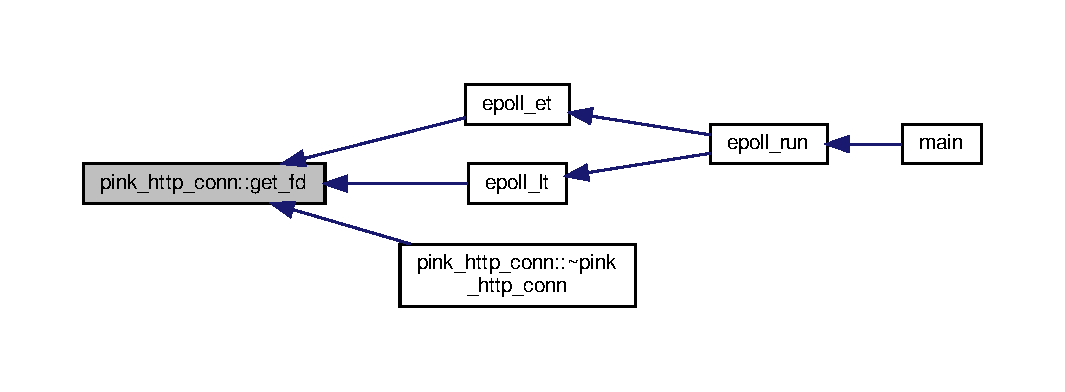
\includegraphics[width=350pt]{classpink__http__conn_aa304899ec9a7f6d7a2a9d738309a9570_icgraph}
\end{center}
\end{figure}
\mbox{\Hypertarget{classpink__http__conn_abff27697496d209cdc7375f99117f018}\label{classpink__http__conn_abff27697496d209cdc7375f99117f018}} 
\index{pink\+\_\+http\+\_\+conn@{pink\+\_\+http\+\_\+conn}!init@{init}}
\index{init@{init}!pink\+\_\+http\+\_\+conn@{pink\+\_\+http\+\_\+conn}}
\subsubsection{\texorpdfstring{init()}{init()}}
{\footnotesize\ttfamily void pink\+\_\+http\+\_\+conn\+::init (\begin{DoxyParamCaption}\item[{int}]{sockfd,  }\item[{const sockaddr\+\_\+in \&}]{addr }\end{DoxyParamCaption})}



Definition at line 25 of file pink\+\_\+http\+\_\+conn.\+cpp.

Here is the call graph for this function\+:
\nopagebreak
\begin{figure}[H]
\begin{center}
\leavevmode
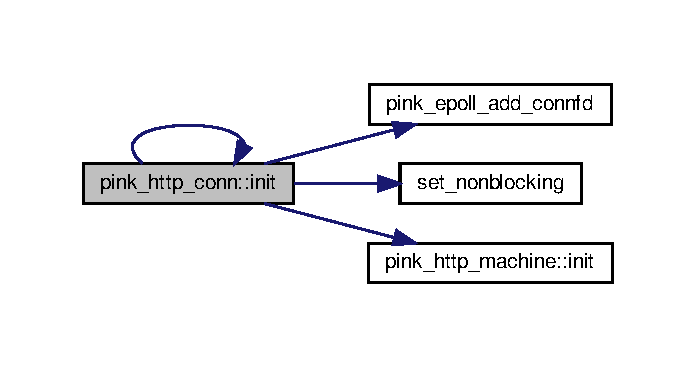
\includegraphics[width=334pt]{classpink__http__conn_abff27697496d209cdc7375f99117f018_cgraph}
\end{center}
\end{figure}
Here is the caller graph for this function\+:
\nopagebreak
\begin{figure}[H]
\begin{center}
\leavevmode
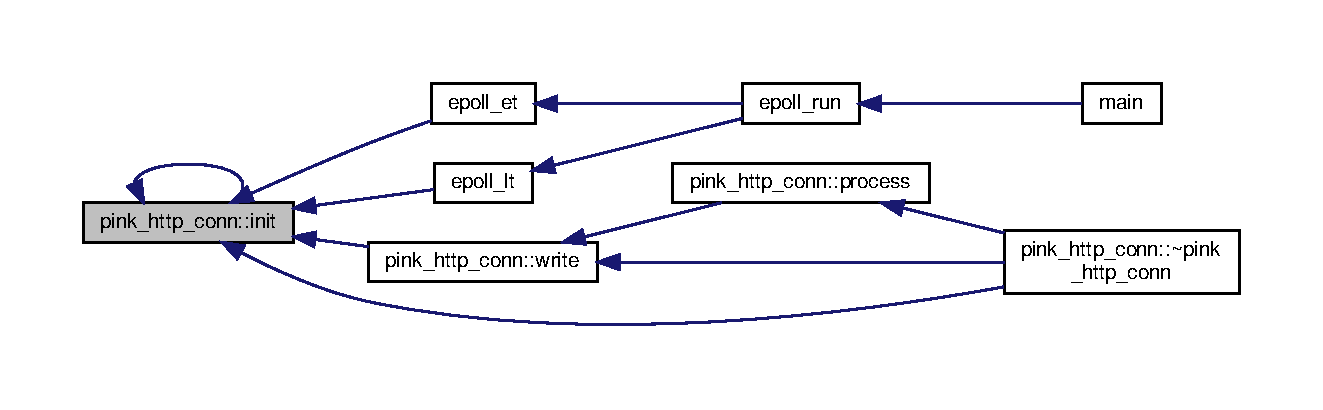
\includegraphics[width=350pt]{classpink__http__conn_abff27697496d209cdc7375f99117f018_icgraph}
\end{center}
\end{figure}
\mbox{\Hypertarget{classpink__http__conn_a14ed30d2643f52ec95c45b11b13b2411}\label{classpink__http__conn_a14ed30d2643f52ec95c45b11b13b2411}} 
\index{pink\+\_\+http\+\_\+conn@{pink\+\_\+http\+\_\+conn}!init\+\_\+listen@{init\+\_\+listen}}
\index{init\+\_\+listen@{init\+\_\+listen}!pink\+\_\+http\+\_\+conn@{pink\+\_\+http\+\_\+conn}}
\subsubsection{\texorpdfstring{init\+\_\+listen()}{init\_listen()}}
{\footnotesize\ttfamily void pink\+\_\+http\+\_\+conn\+::init\+\_\+listen (\begin{DoxyParamCaption}\item[{int}]{sockfd }\end{DoxyParamCaption})}



Definition at line 21 of file pink\+\_\+http\+\_\+conn.\+cpp.

Here is the caller graph for this function\+:
\nopagebreak
\begin{figure}[H]
\begin{center}
\leavevmode
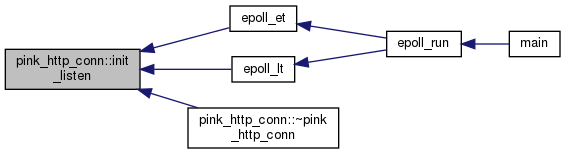
\includegraphics[width=350pt]{classpink__http__conn_a14ed30d2643f52ec95c45b11b13b2411_icgraph}
\end{center}
\end{figure}
\mbox{\Hypertarget{classpink__http__conn_a41ca12d76d0056562633f27d456d0b62}\label{classpink__http__conn_a41ca12d76d0056562633f27d456d0b62}} 
\index{pink\+\_\+http\+\_\+conn@{pink\+\_\+http\+\_\+conn}!process@{process}}
\index{process@{process}!pink\+\_\+http\+\_\+conn@{pink\+\_\+http\+\_\+conn}}
\subsubsection{\texorpdfstring{process()}{process()}}
{\footnotesize\ttfamily void pink\+\_\+http\+\_\+conn\+::process (\begin{DoxyParamCaption}\item[{int}]{flag }\end{DoxyParamCaption})}



Definition at line 54 of file pink\+\_\+http\+\_\+conn.\+cpp.

Here is the call graph for this function\+:
\nopagebreak
\begin{figure}[H]
\begin{center}
\leavevmode
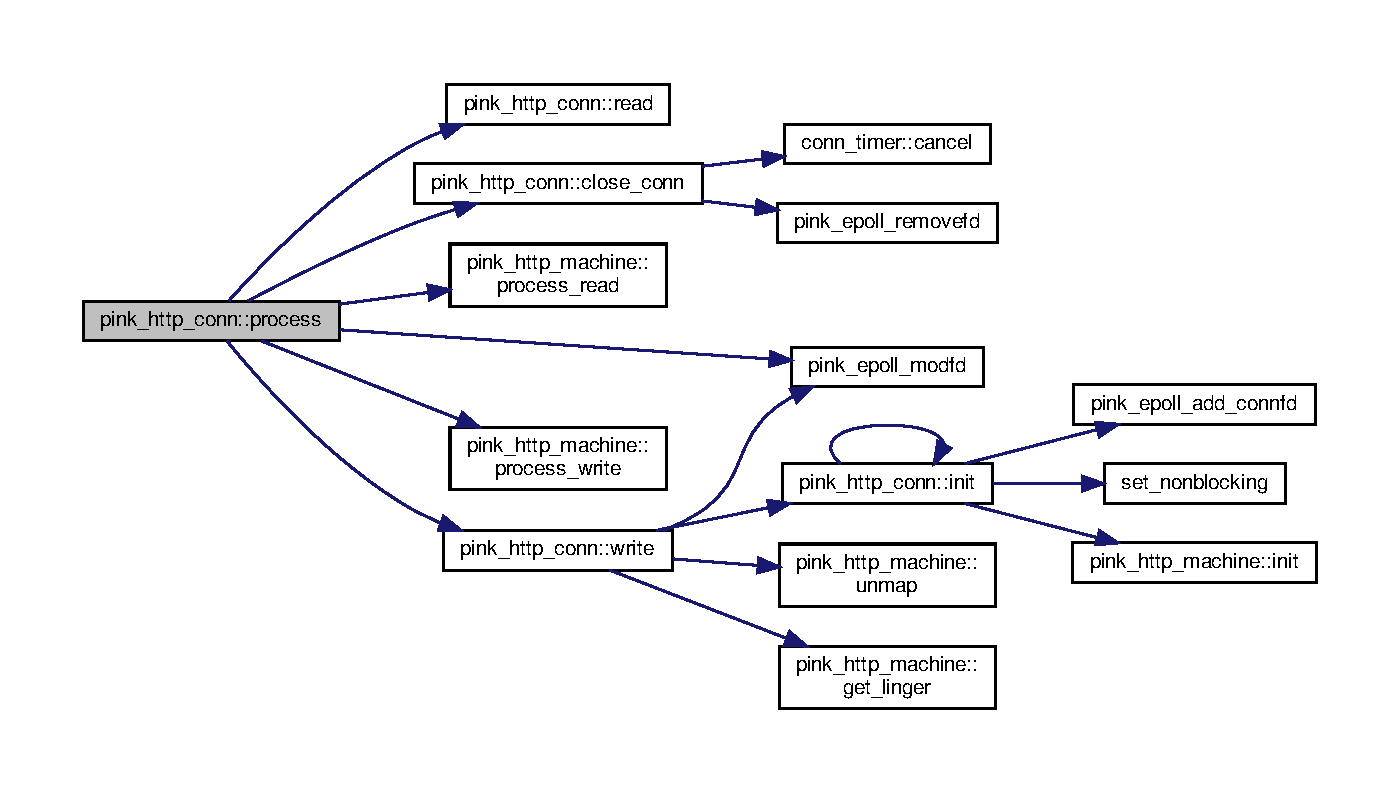
\includegraphics[width=350pt]{classpink__http__conn_a41ca12d76d0056562633f27d456d0b62_cgraph}
\end{center}
\end{figure}
Here is the caller graph for this function\+:
\nopagebreak
\begin{figure}[H]
\begin{center}
\leavevmode
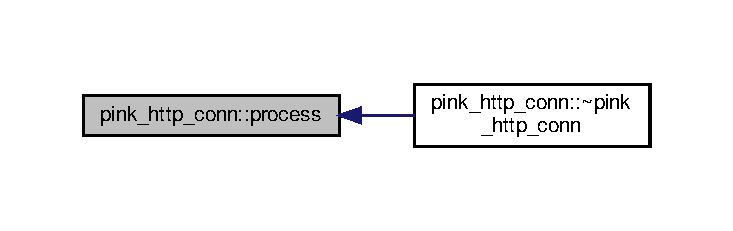
\includegraphics[width=350pt]{classpink__http__conn_a41ca12d76d0056562633f27d456d0b62_icgraph}
\end{center}
\end{figure}
\mbox{\Hypertarget{classpink__http__conn_a254c09e8b962e5a0bc116f8da271b5ed}\label{classpink__http__conn_a254c09e8b962e5a0bc116f8da271b5ed}} 
\index{pink\+\_\+http\+\_\+conn@{pink\+\_\+http\+\_\+conn}!read@{read}}
\index{read@{read}!pink\+\_\+http\+\_\+conn@{pink\+\_\+http\+\_\+conn}}
\subsubsection{\texorpdfstring{read()}{read()}}
{\footnotesize\ttfamily bool pink\+\_\+http\+\_\+conn\+::read (\begin{DoxyParamCaption}{ }\end{DoxyParamCaption})}



Definition at line 87 of file pink\+\_\+http\+\_\+conn.\+cpp.

Here is the caller graph for this function\+:
\nopagebreak
\begin{figure}[H]
\begin{center}
\leavevmode
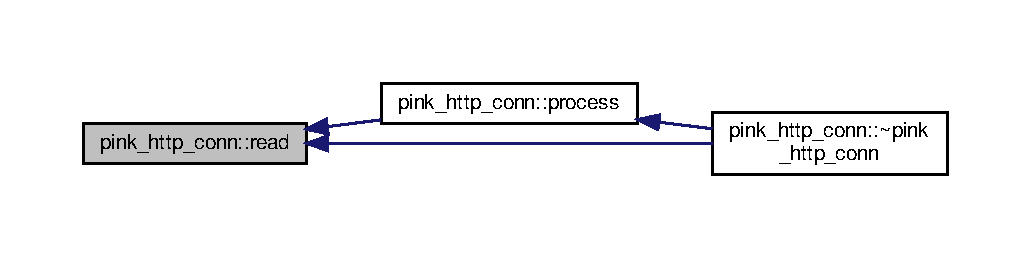
\includegraphics[width=350pt]{classpink__http__conn_a254c09e8b962e5a0bc116f8da271b5ed_icgraph}
\end{center}
\end{figure}
\mbox{\Hypertarget{classpink__http__conn_a362df085394bbf2818c8af93932c80d5}\label{classpink__http__conn_a362df085394bbf2818c8af93932c80d5}} 
\index{pink\+\_\+http\+\_\+conn@{pink\+\_\+http\+\_\+conn}!write@{write}}
\index{write@{write}!pink\+\_\+http\+\_\+conn@{pink\+\_\+http\+\_\+conn}}
\subsubsection{\texorpdfstring{write()}{write()}}
{\footnotesize\ttfamily bool pink\+\_\+http\+\_\+conn\+::write (\begin{DoxyParamCaption}{ }\end{DoxyParamCaption})}



Definition at line 112 of file pink\+\_\+http\+\_\+conn.\+cpp.

Here is the call graph for this function\+:
\nopagebreak
\begin{figure}[H]
\begin{center}
\leavevmode
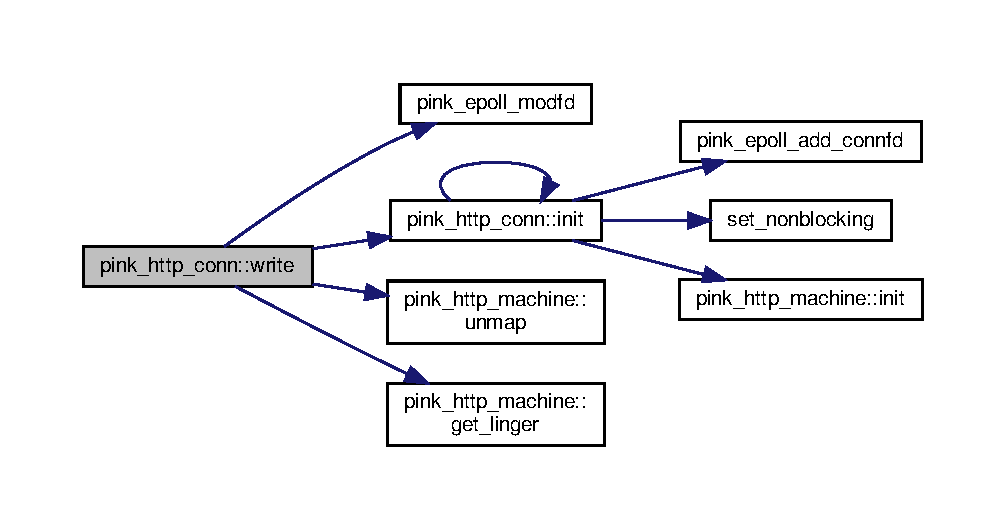
\includegraphics[width=350pt]{classpink__http__conn_a362df085394bbf2818c8af93932c80d5_cgraph}
\end{center}
\end{figure}
Here is the caller graph for this function\+:
\nopagebreak
\begin{figure}[H]
\begin{center}
\leavevmode
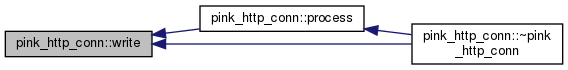
\includegraphics[width=350pt]{classpink__http__conn_a362df085394bbf2818c8af93932c80d5_icgraph}
\end{center}
\end{figure}


\subsection{Member Data Documentation}
\mbox{\Hypertarget{classpink__http__conn_a36a48a19aa593001494eb51106628ebd}\label{classpink__http__conn_a36a48a19aa593001494eb51106628ebd}} 
\index{pink\+\_\+http\+\_\+conn@{pink\+\_\+http\+\_\+conn}!delete\+\_\+cb\+\_\+func@{delete\+\_\+cb\+\_\+func}}
\index{delete\+\_\+cb\+\_\+func@{delete\+\_\+cb\+\_\+func}!pink\+\_\+http\+\_\+conn@{pink\+\_\+http\+\_\+conn}}
\subsubsection{\texorpdfstring{delete\+\_\+cb\+\_\+func}{delete\_cb\_func}}
{\footnotesize\ttfamily void($\ast$ pink\+\_\+http\+\_\+conn\+::delete\+\_\+cb\+\_\+func)(\hyperlink{classpink__http__conn}{pink\+\_\+http\+\_\+conn} $\ast$) = nullptr\hspace{0.3cm}{\ttfamily [static]}}



Definition at line 37 of file pink\+\_\+http\+\_\+conn.\+h.

\mbox{\Hypertarget{classpink__http__conn_a106c011c818e2a80dbb14c61abbe9a2a}\label{classpink__http__conn_a106c011c818e2a80dbb14c61abbe9a2a}} 
\index{pink\+\_\+http\+\_\+conn@{pink\+\_\+http\+\_\+conn}!epollfd@{epollfd}}
\index{epollfd@{epollfd}!pink\+\_\+http\+\_\+conn@{pink\+\_\+http\+\_\+conn}}
\subsubsection{\texorpdfstring{epollfd}{epollfd}}
{\footnotesize\ttfamily int pink\+\_\+http\+\_\+conn\+::epollfd = -\/1\hspace{0.3cm}{\ttfamily [static]}}



Definition at line 46 of file pink\+\_\+http\+\_\+conn.\+h.

\mbox{\Hypertarget{classpink__http__conn_a240ddaa8b2707d66601b1b82c002ef96}\label{classpink__http__conn_a240ddaa8b2707d66601b1b82c002ef96}} 
\index{pink\+\_\+http\+\_\+conn@{pink\+\_\+http\+\_\+conn}!R\+E\+A\+D\+\_\+\+B\+U\+F\+F\+E\+R\+\_\+\+S\+I\+ZE@{R\+E\+A\+D\+\_\+\+B\+U\+F\+F\+E\+R\+\_\+\+S\+I\+ZE}}
\index{R\+E\+A\+D\+\_\+\+B\+U\+F\+F\+E\+R\+\_\+\+S\+I\+ZE@{R\+E\+A\+D\+\_\+\+B\+U\+F\+F\+E\+R\+\_\+\+S\+I\+ZE}!pink\+\_\+http\+\_\+conn@{pink\+\_\+http\+\_\+conn}}
\subsubsection{\texorpdfstring{R\+E\+A\+D\+\_\+\+B\+U\+F\+F\+E\+R\+\_\+\+S\+I\+ZE}{READ\_BUFFER\_SIZE}}
{\footnotesize\ttfamily const int pink\+\_\+http\+\_\+conn\+::\+R\+E\+A\+D\+\_\+\+B\+U\+F\+F\+E\+R\+\_\+\+S\+I\+ZE = 2048\hspace{0.3cm}{\ttfamily [static]}}



Definition at line 44 of file pink\+\_\+http\+\_\+conn.\+h.

\mbox{\Hypertarget{classpink__http__conn_a8687eb679249e4ae085c319dd2d4dfc7}\label{classpink__http__conn_a8687eb679249e4ae085c319dd2d4dfc7}} 
\index{pink\+\_\+http\+\_\+conn@{pink\+\_\+http\+\_\+conn}!timeout@{timeout}}
\index{timeout@{timeout}!pink\+\_\+http\+\_\+conn@{pink\+\_\+http\+\_\+conn}}
\subsubsection{\texorpdfstring{timeout}{timeout}}
{\footnotesize\ttfamily bool pink\+\_\+http\+\_\+conn\+::timeout}



Definition at line 49 of file pink\+\_\+http\+\_\+conn.\+h.

\mbox{\Hypertarget{classpink__http__conn_a0b34c6a8a6b8f65fa882adb109990e43}\label{classpink__http__conn_a0b34c6a8a6b8f65fa882adb109990e43}} 
\index{pink\+\_\+http\+\_\+conn@{pink\+\_\+http\+\_\+conn}!timer@{timer}}
\index{timer@{timer}!pink\+\_\+http\+\_\+conn@{pink\+\_\+http\+\_\+conn}}
\subsubsection{\texorpdfstring{timer}{timer}}
{\footnotesize\ttfamily \hyperlink{classconn__timer}{conn\+\_\+timer}$\ast$ pink\+\_\+http\+\_\+conn\+::timer}



Definition at line 48 of file pink\+\_\+http\+\_\+conn.\+h.

\mbox{\Hypertarget{classpink__http__conn_a4796952e9f7dc2a940e5681bc8f04139}\label{classpink__http__conn_a4796952e9f7dc2a940e5681bc8f04139}} 
\index{pink\+\_\+http\+\_\+conn@{pink\+\_\+http\+\_\+conn}!user\+\_\+count@{user\+\_\+count}}
\index{user\+\_\+count@{user\+\_\+count}!pink\+\_\+http\+\_\+conn@{pink\+\_\+http\+\_\+conn}}
\subsubsection{\texorpdfstring{user\+\_\+count}{user\_count}}
{\footnotesize\ttfamily int pink\+\_\+http\+\_\+conn\+::user\+\_\+count = 0\hspace{0.3cm}{\ttfamily [static]}}



Definition at line 47 of file pink\+\_\+http\+\_\+conn.\+h.

\mbox{\Hypertarget{classpink__http__conn_a7764e0564be1e1ae66c44cf34550efea}\label{classpink__http__conn_a7764e0564be1e1ae66c44cf34550efea}} 
\index{pink\+\_\+http\+\_\+conn@{pink\+\_\+http\+\_\+conn}!W\+R\+I\+T\+E\+\_\+\+B\+U\+F\+F\+E\+R\+\_\+\+S\+I\+ZE@{W\+R\+I\+T\+E\+\_\+\+B\+U\+F\+F\+E\+R\+\_\+\+S\+I\+ZE}}
\index{W\+R\+I\+T\+E\+\_\+\+B\+U\+F\+F\+E\+R\+\_\+\+S\+I\+ZE@{W\+R\+I\+T\+E\+\_\+\+B\+U\+F\+F\+E\+R\+\_\+\+S\+I\+ZE}!pink\+\_\+http\+\_\+conn@{pink\+\_\+http\+\_\+conn}}
\subsubsection{\texorpdfstring{W\+R\+I\+T\+E\+\_\+\+B\+U\+F\+F\+E\+R\+\_\+\+S\+I\+ZE}{WRITE\_BUFFER\_SIZE}}
{\footnotesize\ttfamily const int pink\+\_\+http\+\_\+conn\+::\+W\+R\+I\+T\+E\+\_\+\+B\+U\+F\+F\+E\+R\+\_\+\+S\+I\+ZE = 1024\hspace{0.3cm}{\ttfamily [static]}}



Definition at line 45 of file pink\+\_\+http\+\_\+conn.\+h.



The documentation for this class was generated from the following files\+:\begin{DoxyCompactItemize}
\item 
\hyperlink{pink__http__conn_8h}{pink\+\_\+http\+\_\+conn.\+h}\item 
\hyperlink{pink__http__conn_8cpp}{pink\+\_\+http\+\_\+conn.\+cpp}\end{DoxyCompactItemize}

\hypertarget{classpink__http__machine}{}\section{pink\+\_\+http\+\_\+machine Class Reference}
\label{classpink__http__machine}\index{pink\+\_\+http\+\_\+machine@{pink\+\_\+http\+\_\+machine}}


{\ttfamily \#include $<$pink\+\_\+http\+\_\+machine.\+h$>$}



Collaboration diagram for pink\+\_\+http\+\_\+machine\+:
\nopagebreak
\begin{figure}[H]
\begin{center}
\leavevmode
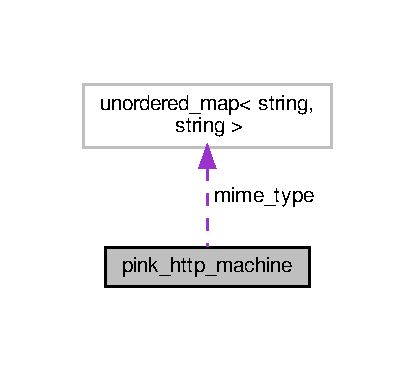
\includegraphics[width=199pt]{classpink__http__machine__coll__graph}
\end{center}
\end{figure}
\subsection*{Public Types}
\begin{DoxyCompactItemize}
\item 
enum \hyperlink{classpink__http__machine_a64bc87fde84112f9e18a09c7d439aa2b}{M\+E\+T\+H\+OD} \{ \newline
\hyperlink{classpink__http__machine_a64bc87fde84112f9e18a09c7d439aa2ba941353ab7fbe8de7c3e211613c832521}{G\+ET} =0, 
\hyperlink{classpink__http__machine_a64bc87fde84112f9e18a09c7d439aa2ba9aac7af48a218454e17ff29dba82f0be}{P\+O\+ST}, 
\hyperlink{classpink__http__machine_a64bc87fde84112f9e18a09c7d439aa2ba32337e87e4cf7dbe8de6241d55b2674b}{H\+E\+AD}, 
\hyperlink{classpink__http__machine_a64bc87fde84112f9e18a09c7d439aa2badee80adbc5551abbeb1bb4c0674f322a}{P\+UT}, 
\newline
\hyperlink{classpink__http__machine_a64bc87fde84112f9e18a09c7d439aa2ba8774cb5bcde90169f21fa72e5d618de7}{D\+E\+L\+E\+TE}, 
\hyperlink{classpink__http__machine_a64bc87fde84112f9e18a09c7d439aa2badcdb9de10fe7689ba1cf313c0de85229}{T\+R\+A\+CE}, 
\hyperlink{classpink__http__machine_a64bc87fde84112f9e18a09c7d439aa2ba0dc30f9df08eed397e07be7cf43af2ea}{O\+P\+T\+I\+O\+NS}, 
\hyperlink{classpink__http__machine_a64bc87fde84112f9e18a09c7d439aa2baeb9d3fcb973b6922d8b1ddb1e6290204}{C\+O\+N\+N\+E\+CT}, 
\newline
\hyperlink{classpink__http__machine_a64bc87fde84112f9e18a09c7d439aa2bad1fda1b7588701be35981d2bdffd3959}{P\+A\+T\+CH}, 
\hyperlink{classpink__http__machine_a64bc87fde84112f9e18a09c7d439aa2bac9ca94619d2ce5c718356d251c7a5127}{U\+N\+K\+N\+O\+W\+N\+\_\+\+M\+E\+T\+H\+OD}
 \}
\item 
enum \hyperlink{classpink__http__machine_aeb5dafe8258708065e5c09565dd37f9e}{C\+H\+E\+C\+K\+\_\+\+S\+T\+A\+TE} \{ \hyperlink{classpink__http__machine_aeb5dafe8258708065e5c09565dd37f9ea45849c7923cca06d5e7a8c2024cb2d1e}{C\+H\+E\+C\+K\+\_\+\+S\+T\+A\+T\+E\+\_\+\+R\+E\+Q\+U\+E\+S\+T\+L\+I\+NE} = 0, 
\hyperlink{classpink__http__machine_aeb5dafe8258708065e5c09565dd37f9eaadc3fa37b117c846fc9bc7b188ce2bfe}{C\+H\+E\+C\+K\+\_\+\+S\+T\+A\+T\+E\+\_\+\+H\+E\+A\+D\+ER}, 
\hyperlink{classpink__http__machine_aeb5dafe8258708065e5c09565dd37f9eac27eaf6929e26d60c742247caf03d0ee}{C\+H\+E\+C\+K\+\_\+\+S\+T\+A\+T\+E\+\_\+\+C\+O\+N\+T\+E\+NT}
 \}
\item 
enum \hyperlink{classpink__http__machine_afb1e590cd61676c2f8859c4e01e5b150}{H\+T\+T\+P\+\_\+\+C\+O\+DE} \{ \newline
\hyperlink{classpink__http__machine_afb1e590cd61676c2f8859c4e01e5b150ab2ca25354e96b87e666a892a1ac8c35c}{N\+O\+T\+\_\+\+C\+O\+M\+P\+L\+E\+T\+ED}, 
\hyperlink{classpink__http__machine_afb1e590cd61676c2f8859c4e01e5b150af80968b6c39c54dff2e5d5541658a374}{G\+E\+T\+\_\+\+R\+E\+Q\+U\+E\+ST}, 
\hyperlink{classpink__http__machine_afb1e590cd61676c2f8859c4e01e5b150a593a224a7435a2c69aec97d827efbb8b}{B\+A\+D\+\_\+\+R\+E\+Q\+U\+E\+ST}, 
\hyperlink{classpink__http__machine_afb1e590cd61676c2f8859c4e01e5b150a0b325eacf5b65952576b6197785e86b9}{N\+O\+\_\+\+R\+E\+S\+O\+U\+R\+CE}, 
\newline
\hyperlink{classpink__http__machine_afb1e590cd61676c2f8859c4e01e5b150aef6f8e15b18fb0bad605acba3ddfd4ad}{F\+O\+R\+B\+I\+D\+D\+E\+N\+\_\+\+R\+E\+Q\+U\+E\+ST}, 
\hyperlink{classpink__http__machine_afb1e590cd61676c2f8859c4e01e5b150a44149cde43145b42953c4825f5d51107}{F\+I\+L\+E\+\_\+\+R\+E\+Q\+U\+E\+ST}, 
\hyperlink{classpink__http__machine_afb1e590cd61676c2f8859c4e01e5b150aa4e2f23c9ddc8e39742256ed3f1725d7}{I\+N\+T\+E\+R\+N\+A\+L\+\_\+\+E\+R\+R\+OR}, 
\hyperlink{classpink__http__machine_afb1e590cd61676c2f8859c4e01e5b150ab3925c78bae06472d9317e9b5e5b68fa}{C\+L\+O\+S\+E\+D\+\_\+\+C\+O\+N\+N\+E\+C\+T\+I\+ON}
 \}
\item 
enum \hyperlink{classpink__http__machine_ab93a9e606b05f96c1b4b0f7079d1e279}{L\+I\+N\+E\+\_\+\+S\+T\+A\+T\+US} \{ \hyperlink{classpink__http__machine_ab93a9e606b05f96c1b4b0f7079d1e279a20dc04aa8adadcff78c8a123f5c311a4}{L\+I\+N\+E\+\_\+\+OK} = 0, 
\hyperlink{classpink__http__machine_ab93a9e606b05f96c1b4b0f7079d1e279a6bf5713029c7f488f44cc8f9ae94ac25}{L\+I\+N\+E\+\_\+\+B\+AD}, 
\hyperlink{classpink__http__machine_ab93a9e606b05f96c1b4b0f7079d1e279a42889372cee61ec858a6ae605284f4f2}{L\+I\+N\+E\+\_\+\+O\+P\+EN}
 \}
\end{DoxyCompactItemize}
\subsection*{Public Member Functions}
\begin{DoxyCompactItemize}
\item 
\hyperlink{classpink__http__machine_a8f5a3d6283cb4e9237cf1deb01548826}{pink\+\_\+http\+\_\+machine} ()
\item 
\hyperlink{classpink__http__machine_a38d1d6228955fc97c752d330d4c126c2}{$\sim$pink\+\_\+http\+\_\+machine} ()
\item 
void \hyperlink{classpink__http__machine_a32b0ee47de1b90467d17194fa83b4eb0}{init} (char $\ast$read\+\_\+buf, char $\ast$write\+\_\+buf, int $\ast$read\+\_\+idx, int $\ast$write\+\_\+idx, const int read\+\_\+buf\+\_\+size, const int write\+\_\+buf\+\_\+size)
\item 
\hyperlink{classpink__http__machine_afb1e590cd61676c2f8859c4e01e5b150}{H\+T\+T\+P\+\_\+\+C\+O\+DE} \hyperlink{classpink__http__machine_a7c937bd8da6bdfbf4894e6af9a712d60}{process\+\_\+read} ()
\item 
bool \hyperlink{classpink__http__machine_a7144e4279cd09ab8ce56873bd3906f24}{process\+\_\+write} (\hyperlink{classpink__http__machine_afb1e590cd61676c2f8859c4e01e5b150}{H\+T\+T\+P\+\_\+\+C\+O\+DE} ret, struct iovec $\ast$iv, int \&iv\+\_\+count)
\item 
void \hyperlink{classpink__http__machine_a26debab8c361df5c79966f11e2b2dd17}{unmap} ()
\item 
bool \hyperlink{classpink__http__machine_a01dcf59a537c21d5a4a92c1c25fbf3ab}{get\+\_\+linger} ()
\end{DoxyCompactItemize}
\subsection*{Static Public Member Functions}
\begin{DoxyCompactItemize}
\item 
static unordered\+\_\+map$<$ string, string $>$ \hyperlink{classpink__http__machine_ad6d404392628f4b2c94a4b30fefb62f8}{mime\+\_\+map\+\_\+init} ()
\end{DoxyCompactItemize}
\subsection*{Static Public Attributes}
\begin{DoxyCompactItemize}
\item 
static constexpr int \hyperlink{classpink__http__machine_a33993ee83910b37ae5672c6e6c94cac3}{F\+I\+L\+E\+N\+A\+M\+E\+\_\+\+L\+EN} = 1024
\item 
static unordered\+\_\+map$<$ string, string $>$ \hyperlink{classpink__http__machine_a4373363c5bd675e182f502d300157aa9}{mime\+\_\+type}
\end{DoxyCompactItemize}


\subsection{Detailed Description}


Definition at line 33 of file pink\+\_\+http\+\_\+machine.\+h.



\subsection{Member Enumeration Documentation}
\mbox{\Hypertarget{classpink__http__machine_aeb5dafe8258708065e5c09565dd37f9e}\label{classpink__http__machine_aeb5dafe8258708065e5c09565dd37f9e}} 
\index{pink\+\_\+http\+\_\+machine@{pink\+\_\+http\+\_\+machine}!C\+H\+E\+C\+K\+\_\+\+S\+T\+A\+TE@{C\+H\+E\+C\+K\+\_\+\+S\+T\+A\+TE}}
\index{C\+H\+E\+C\+K\+\_\+\+S\+T\+A\+TE@{C\+H\+E\+C\+K\+\_\+\+S\+T\+A\+TE}!pink\+\_\+http\+\_\+machine@{pink\+\_\+http\+\_\+machine}}
\subsubsection{\texorpdfstring{C\+H\+E\+C\+K\+\_\+\+S\+T\+A\+TE}{CHECK\_STATE}}
{\footnotesize\ttfamily enum \hyperlink{classpink__http__machine_aeb5dafe8258708065e5c09565dd37f9e}{pink\+\_\+http\+\_\+machine\+::\+C\+H\+E\+C\+K\+\_\+\+S\+T\+A\+TE}}

\begin{DoxyEnumFields}{Enumerator}
\raisebox{\heightof{T}}[0pt][0pt]{\index{C\+H\+E\+C\+K\+\_\+\+S\+T\+A\+T\+E\+\_\+\+R\+E\+Q\+U\+E\+S\+T\+L\+I\+NE@{C\+H\+E\+C\+K\+\_\+\+S\+T\+A\+T\+E\+\_\+\+R\+E\+Q\+U\+E\+S\+T\+L\+I\+NE}!pink\+\_\+http\+\_\+machine@{pink\+\_\+http\+\_\+machine}}\index{pink\+\_\+http\+\_\+machine@{pink\+\_\+http\+\_\+machine}!C\+H\+E\+C\+K\+\_\+\+S\+T\+A\+T\+E\+\_\+\+R\+E\+Q\+U\+E\+S\+T\+L\+I\+NE@{C\+H\+E\+C\+K\+\_\+\+S\+T\+A\+T\+E\+\_\+\+R\+E\+Q\+U\+E\+S\+T\+L\+I\+NE}}}\mbox{\Hypertarget{classpink__http__machine_aeb5dafe8258708065e5c09565dd37f9ea45849c7923cca06d5e7a8c2024cb2d1e}\label{classpink__http__machine_aeb5dafe8258708065e5c09565dd37f9ea45849c7923cca06d5e7a8c2024cb2d1e}} 
C\+H\+E\+C\+K\+\_\+\+S\+T\+A\+T\+E\+\_\+\+R\+E\+Q\+U\+E\+S\+T\+L\+I\+NE&\\
\hline

\raisebox{\heightof{T}}[0pt][0pt]{\index{C\+H\+E\+C\+K\+\_\+\+S\+T\+A\+T\+E\+\_\+\+H\+E\+A\+D\+ER@{C\+H\+E\+C\+K\+\_\+\+S\+T\+A\+T\+E\+\_\+\+H\+E\+A\+D\+ER}!pink\+\_\+http\+\_\+machine@{pink\+\_\+http\+\_\+machine}}\index{pink\+\_\+http\+\_\+machine@{pink\+\_\+http\+\_\+machine}!C\+H\+E\+C\+K\+\_\+\+S\+T\+A\+T\+E\+\_\+\+H\+E\+A\+D\+ER@{C\+H\+E\+C\+K\+\_\+\+S\+T\+A\+T\+E\+\_\+\+H\+E\+A\+D\+ER}}}\mbox{\Hypertarget{classpink__http__machine_aeb5dafe8258708065e5c09565dd37f9eaadc3fa37b117c846fc9bc7b188ce2bfe}\label{classpink__http__machine_aeb5dafe8258708065e5c09565dd37f9eaadc3fa37b117c846fc9bc7b188ce2bfe}} 
C\+H\+E\+C\+K\+\_\+\+S\+T\+A\+T\+E\+\_\+\+H\+E\+A\+D\+ER&\\
\hline

\raisebox{\heightof{T}}[0pt][0pt]{\index{C\+H\+E\+C\+K\+\_\+\+S\+T\+A\+T\+E\+\_\+\+C\+O\+N\+T\+E\+NT@{C\+H\+E\+C\+K\+\_\+\+S\+T\+A\+T\+E\+\_\+\+C\+O\+N\+T\+E\+NT}!pink\+\_\+http\+\_\+machine@{pink\+\_\+http\+\_\+machine}}\index{pink\+\_\+http\+\_\+machine@{pink\+\_\+http\+\_\+machine}!C\+H\+E\+C\+K\+\_\+\+S\+T\+A\+T\+E\+\_\+\+C\+O\+N\+T\+E\+NT@{C\+H\+E\+C\+K\+\_\+\+S\+T\+A\+T\+E\+\_\+\+C\+O\+N\+T\+E\+NT}}}\mbox{\Hypertarget{classpink__http__machine_aeb5dafe8258708065e5c09565dd37f9eac27eaf6929e26d60c742247caf03d0ee}\label{classpink__http__machine_aeb5dafe8258708065e5c09565dd37f9eac27eaf6929e26d60c742247caf03d0ee}} 
C\+H\+E\+C\+K\+\_\+\+S\+T\+A\+T\+E\+\_\+\+C\+O\+N\+T\+E\+NT&\\
\hline

\end{DoxyEnumFields}


Definition at line 40 of file pink\+\_\+http\+\_\+machine.\+h.

\mbox{\Hypertarget{classpink__http__machine_afb1e590cd61676c2f8859c4e01e5b150}\label{classpink__http__machine_afb1e590cd61676c2f8859c4e01e5b150}} 
\index{pink\+\_\+http\+\_\+machine@{pink\+\_\+http\+\_\+machine}!H\+T\+T\+P\+\_\+\+C\+O\+DE@{H\+T\+T\+P\+\_\+\+C\+O\+DE}}
\index{H\+T\+T\+P\+\_\+\+C\+O\+DE@{H\+T\+T\+P\+\_\+\+C\+O\+DE}!pink\+\_\+http\+\_\+machine@{pink\+\_\+http\+\_\+machine}}
\subsubsection{\texorpdfstring{H\+T\+T\+P\+\_\+\+C\+O\+DE}{HTTP\_CODE}}
{\footnotesize\ttfamily enum \hyperlink{classpink__http__machine_afb1e590cd61676c2f8859c4e01e5b150}{pink\+\_\+http\+\_\+machine\+::\+H\+T\+T\+P\+\_\+\+C\+O\+DE}}

\begin{DoxyEnumFields}{Enumerator}
\raisebox{\heightof{T}}[0pt][0pt]{\index{N\+O\+T\+\_\+\+C\+O\+M\+P\+L\+E\+T\+ED@{N\+O\+T\+\_\+\+C\+O\+M\+P\+L\+E\+T\+ED}!pink\+\_\+http\+\_\+machine@{pink\+\_\+http\+\_\+machine}}\index{pink\+\_\+http\+\_\+machine@{pink\+\_\+http\+\_\+machine}!N\+O\+T\+\_\+\+C\+O\+M\+P\+L\+E\+T\+ED@{N\+O\+T\+\_\+\+C\+O\+M\+P\+L\+E\+T\+ED}}}\mbox{\Hypertarget{classpink__http__machine_afb1e590cd61676c2f8859c4e01e5b150ab2ca25354e96b87e666a892a1ac8c35c}\label{classpink__http__machine_afb1e590cd61676c2f8859c4e01e5b150ab2ca25354e96b87e666a892a1ac8c35c}} 
N\+O\+T\+\_\+\+C\+O\+M\+P\+L\+E\+T\+ED&\\
\hline

\raisebox{\heightof{T}}[0pt][0pt]{\index{G\+E\+T\+\_\+\+R\+E\+Q\+U\+E\+ST@{G\+E\+T\+\_\+\+R\+E\+Q\+U\+E\+ST}!pink\+\_\+http\+\_\+machine@{pink\+\_\+http\+\_\+machine}}\index{pink\+\_\+http\+\_\+machine@{pink\+\_\+http\+\_\+machine}!G\+E\+T\+\_\+\+R\+E\+Q\+U\+E\+ST@{G\+E\+T\+\_\+\+R\+E\+Q\+U\+E\+ST}}}\mbox{\Hypertarget{classpink__http__machine_afb1e590cd61676c2f8859c4e01e5b150af80968b6c39c54dff2e5d5541658a374}\label{classpink__http__machine_afb1e590cd61676c2f8859c4e01e5b150af80968b6c39c54dff2e5d5541658a374}} 
G\+E\+T\+\_\+\+R\+E\+Q\+U\+E\+ST&\\
\hline

\raisebox{\heightof{T}}[0pt][0pt]{\index{B\+A\+D\+\_\+\+R\+E\+Q\+U\+E\+ST@{B\+A\+D\+\_\+\+R\+E\+Q\+U\+E\+ST}!pink\+\_\+http\+\_\+machine@{pink\+\_\+http\+\_\+machine}}\index{pink\+\_\+http\+\_\+machine@{pink\+\_\+http\+\_\+machine}!B\+A\+D\+\_\+\+R\+E\+Q\+U\+E\+ST@{B\+A\+D\+\_\+\+R\+E\+Q\+U\+E\+ST}}}\mbox{\Hypertarget{classpink__http__machine_afb1e590cd61676c2f8859c4e01e5b150a593a224a7435a2c69aec97d827efbb8b}\label{classpink__http__machine_afb1e590cd61676c2f8859c4e01e5b150a593a224a7435a2c69aec97d827efbb8b}} 
B\+A\+D\+\_\+\+R\+E\+Q\+U\+E\+ST&\\
\hline

\raisebox{\heightof{T}}[0pt][0pt]{\index{N\+O\+\_\+\+R\+E\+S\+O\+U\+R\+CE@{N\+O\+\_\+\+R\+E\+S\+O\+U\+R\+CE}!pink\+\_\+http\+\_\+machine@{pink\+\_\+http\+\_\+machine}}\index{pink\+\_\+http\+\_\+machine@{pink\+\_\+http\+\_\+machine}!N\+O\+\_\+\+R\+E\+S\+O\+U\+R\+CE@{N\+O\+\_\+\+R\+E\+S\+O\+U\+R\+CE}}}\mbox{\Hypertarget{classpink__http__machine_afb1e590cd61676c2f8859c4e01e5b150a0b325eacf5b65952576b6197785e86b9}\label{classpink__http__machine_afb1e590cd61676c2f8859c4e01e5b150a0b325eacf5b65952576b6197785e86b9}} 
N\+O\+\_\+\+R\+E\+S\+O\+U\+R\+CE&\\
\hline

\raisebox{\heightof{T}}[0pt][0pt]{\index{F\+O\+R\+B\+I\+D\+D\+E\+N\+\_\+\+R\+E\+Q\+U\+E\+ST@{F\+O\+R\+B\+I\+D\+D\+E\+N\+\_\+\+R\+E\+Q\+U\+E\+ST}!pink\+\_\+http\+\_\+machine@{pink\+\_\+http\+\_\+machine}}\index{pink\+\_\+http\+\_\+machine@{pink\+\_\+http\+\_\+machine}!F\+O\+R\+B\+I\+D\+D\+E\+N\+\_\+\+R\+E\+Q\+U\+E\+ST@{F\+O\+R\+B\+I\+D\+D\+E\+N\+\_\+\+R\+E\+Q\+U\+E\+ST}}}\mbox{\Hypertarget{classpink__http__machine_afb1e590cd61676c2f8859c4e01e5b150aef6f8e15b18fb0bad605acba3ddfd4ad}\label{classpink__http__machine_afb1e590cd61676c2f8859c4e01e5b150aef6f8e15b18fb0bad605acba3ddfd4ad}} 
F\+O\+R\+B\+I\+D\+D\+E\+N\+\_\+\+R\+E\+Q\+U\+E\+ST&\\
\hline

\raisebox{\heightof{T}}[0pt][0pt]{\index{F\+I\+L\+E\+\_\+\+R\+E\+Q\+U\+E\+ST@{F\+I\+L\+E\+\_\+\+R\+E\+Q\+U\+E\+ST}!pink\+\_\+http\+\_\+machine@{pink\+\_\+http\+\_\+machine}}\index{pink\+\_\+http\+\_\+machine@{pink\+\_\+http\+\_\+machine}!F\+I\+L\+E\+\_\+\+R\+E\+Q\+U\+E\+ST@{F\+I\+L\+E\+\_\+\+R\+E\+Q\+U\+E\+ST}}}\mbox{\Hypertarget{classpink__http__machine_afb1e590cd61676c2f8859c4e01e5b150a44149cde43145b42953c4825f5d51107}\label{classpink__http__machine_afb1e590cd61676c2f8859c4e01e5b150a44149cde43145b42953c4825f5d51107}} 
F\+I\+L\+E\+\_\+\+R\+E\+Q\+U\+E\+ST&\\
\hline

\raisebox{\heightof{T}}[0pt][0pt]{\index{I\+N\+T\+E\+R\+N\+A\+L\+\_\+\+E\+R\+R\+OR@{I\+N\+T\+E\+R\+N\+A\+L\+\_\+\+E\+R\+R\+OR}!pink\+\_\+http\+\_\+machine@{pink\+\_\+http\+\_\+machine}}\index{pink\+\_\+http\+\_\+machine@{pink\+\_\+http\+\_\+machine}!I\+N\+T\+E\+R\+N\+A\+L\+\_\+\+E\+R\+R\+OR@{I\+N\+T\+E\+R\+N\+A\+L\+\_\+\+E\+R\+R\+OR}}}\mbox{\Hypertarget{classpink__http__machine_afb1e590cd61676c2f8859c4e01e5b150aa4e2f23c9ddc8e39742256ed3f1725d7}\label{classpink__http__machine_afb1e590cd61676c2f8859c4e01e5b150aa4e2f23c9ddc8e39742256ed3f1725d7}} 
I\+N\+T\+E\+R\+N\+A\+L\+\_\+\+E\+R\+R\+OR&\\
\hline

\raisebox{\heightof{T}}[0pt][0pt]{\index{C\+L\+O\+S\+E\+D\+\_\+\+C\+O\+N\+N\+E\+C\+T\+I\+ON@{C\+L\+O\+S\+E\+D\+\_\+\+C\+O\+N\+N\+E\+C\+T\+I\+ON}!pink\+\_\+http\+\_\+machine@{pink\+\_\+http\+\_\+machine}}\index{pink\+\_\+http\+\_\+machine@{pink\+\_\+http\+\_\+machine}!C\+L\+O\+S\+E\+D\+\_\+\+C\+O\+N\+N\+E\+C\+T\+I\+ON@{C\+L\+O\+S\+E\+D\+\_\+\+C\+O\+N\+N\+E\+C\+T\+I\+ON}}}\mbox{\Hypertarget{classpink__http__machine_afb1e590cd61676c2f8859c4e01e5b150ab3925c78bae06472d9317e9b5e5b68fa}\label{classpink__http__machine_afb1e590cd61676c2f8859c4e01e5b150ab3925c78bae06472d9317e9b5e5b68fa}} 
C\+L\+O\+S\+E\+D\+\_\+\+C\+O\+N\+N\+E\+C\+T\+I\+ON&\\
\hline

\end{DoxyEnumFields}


Definition at line 45 of file pink\+\_\+http\+\_\+machine.\+h.

\mbox{\Hypertarget{classpink__http__machine_ab93a9e606b05f96c1b4b0f7079d1e279}\label{classpink__http__machine_ab93a9e606b05f96c1b4b0f7079d1e279}} 
\index{pink\+\_\+http\+\_\+machine@{pink\+\_\+http\+\_\+machine}!L\+I\+N\+E\+\_\+\+S\+T\+A\+T\+US@{L\+I\+N\+E\+\_\+\+S\+T\+A\+T\+US}}
\index{L\+I\+N\+E\+\_\+\+S\+T\+A\+T\+US@{L\+I\+N\+E\+\_\+\+S\+T\+A\+T\+US}!pink\+\_\+http\+\_\+machine@{pink\+\_\+http\+\_\+machine}}
\subsubsection{\texorpdfstring{L\+I\+N\+E\+\_\+\+S\+T\+A\+T\+US}{LINE\_STATUS}}
{\footnotesize\ttfamily enum \hyperlink{classpink__http__machine_ab93a9e606b05f96c1b4b0f7079d1e279}{pink\+\_\+http\+\_\+machine\+::\+L\+I\+N\+E\+\_\+\+S\+T\+A\+T\+US}}

\begin{DoxyEnumFields}{Enumerator}
\raisebox{\heightof{T}}[0pt][0pt]{\index{L\+I\+N\+E\+\_\+\+OK@{L\+I\+N\+E\+\_\+\+OK}!pink\+\_\+http\+\_\+machine@{pink\+\_\+http\+\_\+machine}}\index{pink\+\_\+http\+\_\+machine@{pink\+\_\+http\+\_\+machine}!L\+I\+N\+E\+\_\+\+OK@{L\+I\+N\+E\+\_\+\+OK}}}\mbox{\Hypertarget{classpink__http__machine_ab93a9e606b05f96c1b4b0f7079d1e279a20dc04aa8adadcff78c8a123f5c311a4}\label{classpink__http__machine_ab93a9e606b05f96c1b4b0f7079d1e279a20dc04aa8adadcff78c8a123f5c311a4}} 
L\+I\+N\+E\+\_\+\+OK&\\
\hline

\raisebox{\heightof{T}}[0pt][0pt]{\index{L\+I\+N\+E\+\_\+\+B\+AD@{L\+I\+N\+E\+\_\+\+B\+AD}!pink\+\_\+http\+\_\+machine@{pink\+\_\+http\+\_\+machine}}\index{pink\+\_\+http\+\_\+machine@{pink\+\_\+http\+\_\+machine}!L\+I\+N\+E\+\_\+\+B\+AD@{L\+I\+N\+E\+\_\+\+B\+AD}}}\mbox{\Hypertarget{classpink__http__machine_ab93a9e606b05f96c1b4b0f7079d1e279a6bf5713029c7f488f44cc8f9ae94ac25}\label{classpink__http__machine_ab93a9e606b05f96c1b4b0f7079d1e279a6bf5713029c7f488f44cc8f9ae94ac25}} 
L\+I\+N\+E\+\_\+\+B\+AD&\\
\hline

\raisebox{\heightof{T}}[0pt][0pt]{\index{L\+I\+N\+E\+\_\+\+O\+P\+EN@{L\+I\+N\+E\+\_\+\+O\+P\+EN}!pink\+\_\+http\+\_\+machine@{pink\+\_\+http\+\_\+machine}}\index{pink\+\_\+http\+\_\+machine@{pink\+\_\+http\+\_\+machine}!L\+I\+N\+E\+\_\+\+O\+P\+EN@{L\+I\+N\+E\+\_\+\+O\+P\+EN}}}\mbox{\Hypertarget{classpink__http__machine_ab93a9e606b05f96c1b4b0f7079d1e279a42889372cee61ec858a6ae605284f4f2}\label{classpink__http__machine_ab93a9e606b05f96c1b4b0f7079d1e279a42889372cee61ec858a6ae605284f4f2}} 
L\+I\+N\+E\+\_\+\+O\+P\+EN&\\
\hline

\end{DoxyEnumFields}


Definition at line 49 of file pink\+\_\+http\+\_\+machine.\+h.

\mbox{\Hypertarget{classpink__http__machine_a64bc87fde84112f9e18a09c7d439aa2b}\label{classpink__http__machine_a64bc87fde84112f9e18a09c7d439aa2b}} 
\index{pink\+\_\+http\+\_\+machine@{pink\+\_\+http\+\_\+machine}!M\+E\+T\+H\+OD@{M\+E\+T\+H\+OD}}
\index{M\+E\+T\+H\+OD@{M\+E\+T\+H\+OD}!pink\+\_\+http\+\_\+machine@{pink\+\_\+http\+\_\+machine}}
\subsubsection{\texorpdfstring{M\+E\+T\+H\+OD}{METHOD}}
{\footnotesize\ttfamily enum \hyperlink{classpink__http__machine_a64bc87fde84112f9e18a09c7d439aa2b}{pink\+\_\+http\+\_\+machine\+::\+M\+E\+T\+H\+OD}}

\begin{DoxyEnumFields}{Enumerator}
\raisebox{\heightof{T}}[0pt][0pt]{\index{G\+ET@{G\+ET}!pink\+\_\+http\+\_\+machine@{pink\+\_\+http\+\_\+machine}}\index{pink\+\_\+http\+\_\+machine@{pink\+\_\+http\+\_\+machine}!G\+ET@{G\+ET}}}\mbox{\Hypertarget{classpink__http__machine_a64bc87fde84112f9e18a09c7d439aa2ba941353ab7fbe8de7c3e211613c832521}\label{classpink__http__machine_a64bc87fde84112f9e18a09c7d439aa2ba941353ab7fbe8de7c3e211613c832521}} 
G\+ET&\\
\hline

\raisebox{\heightof{T}}[0pt][0pt]{\index{P\+O\+ST@{P\+O\+ST}!pink\+\_\+http\+\_\+machine@{pink\+\_\+http\+\_\+machine}}\index{pink\+\_\+http\+\_\+machine@{pink\+\_\+http\+\_\+machine}!P\+O\+ST@{P\+O\+ST}}}\mbox{\Hypertarget{classpink__http__machine_a64bc87fde84112f9e18a09c7d439aa2ba9aac7af48a218454e17ff29dba82f0be}\label{classpink__http__machine_a64bc87fde84112f9e18a09c7d439aa2ba9aac7af48a218454e17ff29dba82f0be}} 
P\+O\+ST&\\
\hline

\raisebox{\heightof{T}}[0pt][0pt]{\index{H\+E\+AD@{H\+E\+AD}!pink\+\_\+http\+\_\+machine@{pink\+\_\+http\+\_\+machine}}\index{pink\+\_\+http\+\_\+machine@{pink\+\_\+http\+\_\+machine}!H\+E\+AD@{H\+E\+AD}}}\mbox{\Hypertarget{classpink__http__machine_a64bc87fde84112f9e18a09c7d439aa2ba32337e87e4cf7dbe8de6241d55b2674b}\label{classpink__http__machine_a64bc87fde84112f9e18a09c7d439aa2ba32337e87e4cf7dbe8de6241d55b2674b}} 
H\+E\+AD&\\
\hline

\raisebox{\heightof{T}}[0pt][0pt]{\index{P\+UT@{P\+UT}!pink\+\_\+http\+\_\+machine@{pink\+\_\+http\+\_\+machine}}\index{pink\+\_\+http\+\_\+machine@{pink\+\_\+http\+\_\+machine}!P\+UT@{P\+UT}}}\mbox{\Hypertarget{classpink__http__machine_a64bc87fde84112f9e18a09c7d439aa2badee80adbc5551abbeb1bb4c0674f322a}\label{classpink__http__machine_a64bc87fde84112f9e18a09c7d439aa2badee80adbc5551abbeb1bb4c0674f322a}} 
P\+UT&\\
\hline

\raisebox{\heightof{T}}[0pt][0pt]{\index{D\+E\+L\+E\+TE@{D\+E\+L\+E\+TE}!pink\+\_\+http\+\_\+machine@{pink\+\_\+http\+\_\+machine}}\index{pink\+\_\+http\+\_\+machine@{pink\+\_\+http\+\_\+machine}!D\+E\+L\+E\+TE@{D\+E\+L\+E\+TE}}}\mbox{\Hypertarget{classpink__http__machine_a64bc87fde84112f9e18a09c7d439aa2ba8774cb5bcde90169f21fa72e5d618de7}\label{classpink__http__machine_a64bc87fde84112f9e18a09c7d439aa2ba8774cb5bcde90169f21fa72e5d618de7}} 
D\+E\+L\+E\+TE&\\
\hline

\raisebox{\heightof{T}}[0pt][0pt]{\index{T\+R\+A\+CE@{T\+R\+A\+CE}!pink\+\_\+http\+\_\+machine@{pink\+\_\+http\+\_\+machine}}\index{pink\+\_\+http\+\_\+machine@{pink\+\_\+http\+\_\+machine}!T\+R\+A\+CE@{T\+R\+A\+CE}}}\mbox{\Hypertarget{classpink__http__machine_a64bc87fde84112f9e18a09c7d439aa2badcdb9de10fe7689ba1cf313c0de85229}\label{classpink__http__machine_a64bc87fde84112f9e18a09c7d439aa2badcdb9de10fe7689ba1cf313c0de85229}} 
T\+R\+A\+CE&\\
\hline

\raisebox{\heightof{T}}[0pt][0pt]{\index{O\+P\+T\+I\+O\+NS@{O\+P\+T\+I\+O\+NS}!pink\+\_\+http\+\_\+machine@{pink\+\_\+http\+\_\+machine}}\index{pink\+\_\+http\+\_\+machine@{pink\+\_\+http\+\_\+machine}!O\+P\+T\+I\+O\+NS@{O\+P\+T\+I\+O\+NS}}}\mbox{\Hypertarget{classpink__http__machine_a64bc87fde84112f9e18a09c7d439aa2ba0dc30f9df08eed397e07be7cf43af2ea}\label{classpink__http__machine_a64bc87fde84112f9e18a09c7d439aa2ba0dc30f9df08eed397e07be7cf43af2ea}} 
O\+P\+T\+I\+O\+NS&\\
\hline

\raisebox{\heightof{T}}[0pt][0pt]{\index{C\+O\+N\+N\+E\+CT@{C\+O\+N\+N\+E\+CT}!pink\+\_\+http\+\_\+machine@{pink\+\_\+http\+\_\+machine}}\index{pink\+\_\+http\+\_\+machine@{pink\+\_\+http\+\_\+machine}!C\+O\+N\+N\+E\+CT@{C\+O\+N\+N\+E\+CT}}}\mbox{\Hypertarget{classpink__http__machine_a64bc87fde84112f9e18a09c7d439aa2baeb9d3fcb973b6922d8b1ddb1e6290204}\label{classpink__http__machine_a64bc87fde84112f9e18a09c7d439aa2baeb9d3fcb973b6922d8b1ddb1e6290204}} 
C\+O\+N\+N\+E\+CT&\\
\hline

\raisebox{\heightof{T}}[0pt][0pt]{\index{P\+A\+T\+CH@{P\+A\+T\+CH}!pink\+\_\+http\+\_\+machine@{pink\+\_\+http\+\_\+machine}}\index{pink\+\_\+http\+\_\+machine@{pink\+\_\+http\+\_\+machine}!P\+A\+T\+CH@{P\+A\+T\+CH}}}\mbox{\Hypertarget{classpink__http__machine_a64bc87fde84112f9e18a09c7d439aa2bad1fda1b7588701be35981d2bdffd3959}\label{classpink__http__machine_a64bc87fde84112f9e18a09c7d439aa2bad1fda1b7588701be35981d2bdffd3959}} 
P\+A\+T\+CH&\\
\hline

\raisebox{\heightof{T}}[0pt][0pt]{\index{U\+N\+K\+N\+O\+W\+N\+\_\+\+M\+E\+T\+H\+OD@{U\+N\+K\+N\+O\+W\+N\+\_\+\+M\+E\+T\+H\+OD}!pink\+\_\+http\+\_\+machine@{pink\+\_\+http\+\_\+machine}}\index{pink\+\_\+http\+\_\+machine@{pink\+\_\+http\+\_\+machine}!U\+N\+K\+N\+O\+W\+N\+\_\+\+M\+E\+T\+H\+OD@{U\+N\+K\+N\+O\+W\+N\+\_\+\+M\+E\+T\+H\+OD}}}\mbox{\Hypertarget{classpink__http__machine_a64bc87fde84112f9e18a09c7d439aa2bac9ca94619d2ce5c718356d251c7a5127}\label{classpink__http__machine_a64bc87fde84112f9e18a09c7d439aa2bac9ca94619d2ce5c718356d251c7a5127}} 
U\+N\+K\+N\+O\+W\+N\+\_\+\+M\+E\+T\+H\+OD&\\
\hline

\end{DoxyEnumFields}


Definition at line 36 of file pink\+\_\+http\+\_\+machine.\+h.



\subsection{Constructor \& Destructor Documentation}
\mbox{\Hypertarget{classpink__http__machine_a8f5a3d6283cb4e9237cf1deb01548826}\label{classpink__http__machine_a8f5a3d6283cb4e9237cf1deb01548826}} 
\index{pink\+\_\+http\+\_\+machine@{pink\+\_\+http\+\_\+machine}!pink\+\_\+http\+\_\+machine@{pink\+\_\+http\+\_\+machine}}
\index{pink\+\_\+http\+\_\+machine@{pink\+\_\+http\+\_\+machine}!pink\+\_\+http\+\_\+machine@{pink\+\_\+http\+\_\+machine}}
\subsubsection{\texorpdfstring{pink\+\_\+http\+\_\+machine()}{pink\_http\_machine()}}
{\footnotesize\ttfamily pink\+\_\+http\+\_\+machine\+::pink\+\_\+http\+\_\+machine (\begin{DoxyParamCaption}{ }\end{DoxyParamCaption})\hspace{0.3cm}{\ttfamily [inline]}}



Definition at line 52 of file pink\+\_\+http\+\_\+machine.\+h.

\mbox{\Hypertarget{classpink__http__machine_a38d1d6228955fc97c752d330d4c126c2}\label{classpink__http__machine_a38d1d6228955fc97c752d330d4c126c2}} 
\index{pink\+\_\+http\+\_\+machine@{pink\+\_\+http\+\_\+machine}!````~pink\+\_\+http\+\_\+machine@{$\sim$pink\+\_\+http\+\_\+machine}}
\index{````~pink\+\_\+http\+\_\+machine@{$\sim$pink\+\_\+http\+\_\+machine}!pink\+\_\+http\+\_\+machine@{pink\+\_\+http\+\_\+machine}}
\subsubsection{\texorpdfstring{$\sim$pink\+\_\+http\+\_\+machine()}{~pink\_http\_machine()}}
{\footnotesize\ttfamily pink\+\_\+http\+\_\+machine\+::$\sim$pink\+\_\+http\+\_\+machine (\begin{DoxyParamCaption}{ }\end{DoxyParamCaption})\hspace{0.3cm}{\ttfamily [inline]}}



Definition at line 53 of file pink\+\_\+http\+\_\+machine.\+h.

Here is the call graph for this function\+:
\nopagebreak
\begin{figure}[H]
\begin{center}
\leavevmode
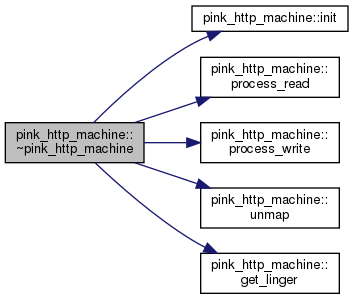
\includegraphics[width=337pt]{classpink__http__machine_a38d1d6228955fc97c752d330d4c126c2_cgraph}
\end{center}
\end{figure}


\subsection{Member Function Documentation}
\mbox{\Hypertarget{classpink__http__machine_a01dcf59a537c21d5a4a92c1c25fbf3ab}\label{classpink__http__machine_a01dcf59a537c21d5a4a92c1c25fbf3ab}} 
\index{pink\+\_\+http\+\_\+machine@{pink\+\_\+http\+\_\+machine}!get\+\_\+linger@{get\+\_\+linger}}
\index{get\+\_\+linger@{get\+\_\+linger}!pink\+\_\+http\+\_\+machine@{pink\+\_\+http\+\_\+machine}}
\subsubsection{\texorpdfstring{get\+\_\+linger()}{get\_linger()}}
{\footnotesize\ttfamily bool pink\+\_\+http\+\_\+machine\+::get\+\_\+linger (\begin{DoxyParamCaption}{ }\end{DoxyParamCaption})}



Definition at line 515 of file pink\+\_\+http\+\_\+machine.\+cpp.

Here is the caller graph for this function\+:
\nopagebreak
\begin{figure}[H]
\begin{center}
\leavevmode
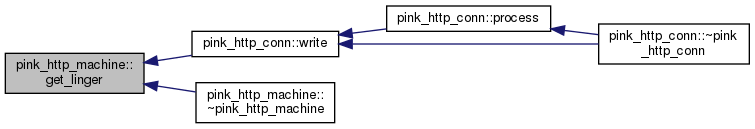
\includegraphics[width=350pt]{classpink__http__machine_a01dcf59a537c21d5a4a92c1c25fbf3ab_icgraph}
\end{center}
\end{figure}
\mbox{\Hypertarget{classpink__http__machine_a32b0ee47de1b90467d17194fa83b4eb0}\label{classpink__http__machine_a32b0ee47de1b90467d17194fa83b4eb0}} 
\index{pink\+\_\+http\+\_\+machine@{pink\+\_\+http\+\_\+machine}!init@{init}}
\index{init@{init}!pink\+\_\+http\+\_\+machine@{pink\+\_\+http\+\_\+machine}}
\subsubsection{\texorpdfstring{init()}{init()}}
{\footnotesize\ttfamily void pink\+\_\+http\+\_\+machine\+::init (\begin{DoxyParamCaption}\item[{char $\ast$}]{read\+\_\+buf,  }\item[{char $\ast$}]{write\+\_\+buf,  }\item[{int $\ast$}]{read\+\_\+idx,  }\item[{int $\ast$}]{write\+\_\+idx,  }\item[{const int}]{read\+\_\+buf\+\_\+size,  }\item[{const int}]{write\+\_\+buf\+\_\+size }\end{DoxyParamCaption})}



Definition at line 63 of file pink\+\_\+http\+\_\+machine.\+cpp.

Here is the caller graph for this function\+:
\nopagebreak
\begin{figure}[H]
\begin{center}
\leavevmode
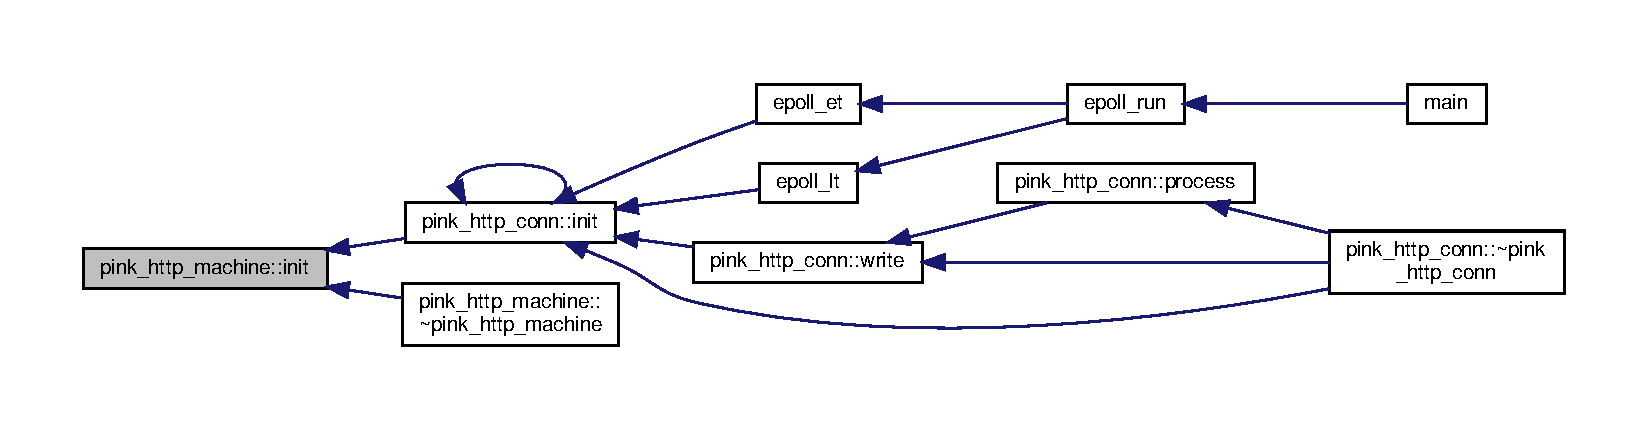
\includegraphics[width=350pt]{classpink__http__machine_a32b0ee47de1b90467d17194fa83b4eb0_icgraph}
\end{center}
\end{figure}
\mbox{\Hypertarget{classpink__http__machine_ad6d404392628f4b2c94a4b30fefb62f8}\label{classpink__http__machine_ad6d404392628f4b2c94a4b30fefb62f8}} 
\index{pink\+\_\+http\+\_\+machine@{pink\+\_\+http\+\_\+machine}!mime\+\_\+map\+\_\+init@{mime\+\_\+map\+\_\+init}}
\index{mime\+\_\+map\+\_\+init@{mime\+\_\+map\+\_\+init}!pink\+\_\+http\+\_\+machine@{pink\+\_\+http\+\_\+machine}}
\subsubsection{\texorpdfstring{mime\+\_\+map\+\_\+init()}{mime\_map\_init()}}
{\footnotesize\ttfamily std\+::unordered\+\_\+map$<$ string, string $>$ pink\+\_\+http\+\_\+machine\+::mime\+\_\+map\+\_\+init (\begin{DoxyParamCaption}{ }\end{DoxyParamCaption})\hspace{0.3cm}{\ttfamily [static]}}



Definition at line 26 of file pink\+\_\+http\+\_\+machine.\+cpp.

\mbox{\Hypertarget{classpink__http__machine_a7c937bd8da6bdfbf4894e6af9a712d60}\label{classpink__http__machine_a7c937bd8da6bdfbf4894e6af9a712d60}} 
\index{pink\+\_\+http\+\_\+machine@{pink\+\_\+http\+\_\+machine}!process\+\_\+read@{process\+\_\+read}}
\index{process\+\_\+read@{process\+\_\+read}!pink\+\_\+http\+\_\+machine@{pink\+\_\+http\+\_\+machine}}
\subsubsection{\texorpdfstring{process\+\_\+read()}{process\_read()}}
{\footnotesize\ttfamily \hyperlink{classpink__http__machine_afb1e590cd61676c2f8859c4e01e5b150}{pink\+\_\+http\+\_\+machine\+::\+H\+T\+T\+P\+\_\+\+C\+O\+DE} pink\+\_\+http\+\_\+machine\+::process\+\_\+read (\begin{DoxyParamCaption}{ }\end{DoxyParamCaption})}



Definition at line 101 of file pink\+\_\+http\+\_\+machine.\+cpp.

Here is the caller graph for this function\+:
\nopagebreak
\begin{figure}[H]
\begin{center}
\leavevmode
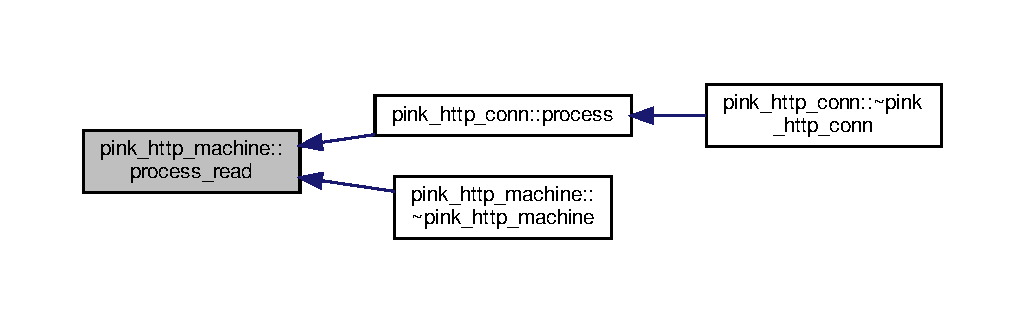
\includegraphics[width=350pt]{classpink__http__machine_a7c937bd8da6bdfbf4894e6af9a712d60_icgraph}
\end{center}
\end{figure}
\mbox{\Hypertarget{classpink__http__machine_a7144e4279cd09ab8ce56873bd3906f24}\label{classpink__http__machine_a7144e4279cd09ab8ce56873bd3906f24}} 
\index{pink\+\_\+http\+\_\+machine@{pink\+\_\+http\+\_\+machine}!process\+\_\+write@{process\+\_\+write}}
\index{process\+\_\+write@{process\+\_\+write}!pink\+\_\+http\+\_\+machine@{pink\+\_\+http\+\_\+machine}}
\subsubsection{\texorpdfstring{process\+\_\+write()}{process\_write()}}
{\footnotesize\ttfamily bool pink\+\_\+http\+\_\+machine\+::process\+\_\+write (\begin{DoxyParamCaption}\item[{\hyperlink{classpink__http__machine_afb1e590cd61676c2f8859c4e01e5b150}{H\+T\+T\+P\+\_\+\+C\+O\+DE}}]{ret,  }\item[{struct iovec $\ast$}]{iv,  }\item[{int \&}]{iv\+\_\+count }\end{DoxyParamCaption})}



Definition at line 394 of file pink\+\_\+http\+\_\+machine.\+cpp.

Here is the caller graph for this function\+:
\nopagebreak
\begin{figure}[H]
\begin{center}
\leavevmode
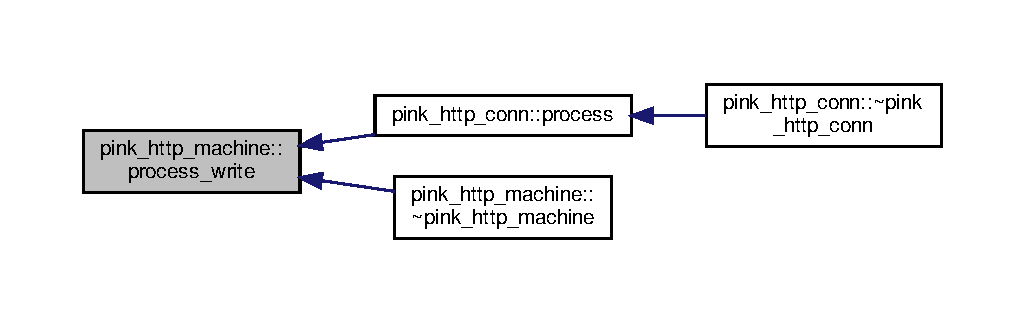
\includegraphics[width=350pt]{classpink__http__machine_a7144e4279cd09ab8ce56873bd3906f24_icgraph}
\end{center}
\end{figure}
\mbox{\Hypertarget{classpink__http__machine_a26debab8c361df5c79966f11e2b2dd17}\label{classpink__http__machine_a26debab8c361df5c79966f11e2b2dd17}} 
\index{pink\+\_\+http\+\_\+machine@{pink\+\_\+http\+\_\+machine}!unmap@{unmap}}
\index{unmap@{unmap}!pink\+\_\+http\+\_\+machine@{pink\+\_\+http\+\_\+machine}}
\subsubsection{\texorpdfstring{unmap()}{unmap()}}
{\footnotesize\ttfamily void pink\+\_\+http\+\_\+machine\+::unmap (\begin{DoxyParamCaption}{ }\end{DoxyParamCaption})}



Definition at line 519 of file pink\+\_\+http\+\_\+machine.\+cpp.

Here is the caller graph for this function\+:
\nopagebreak
\begin{figure}[H]
\begin{center}
\leavevmode
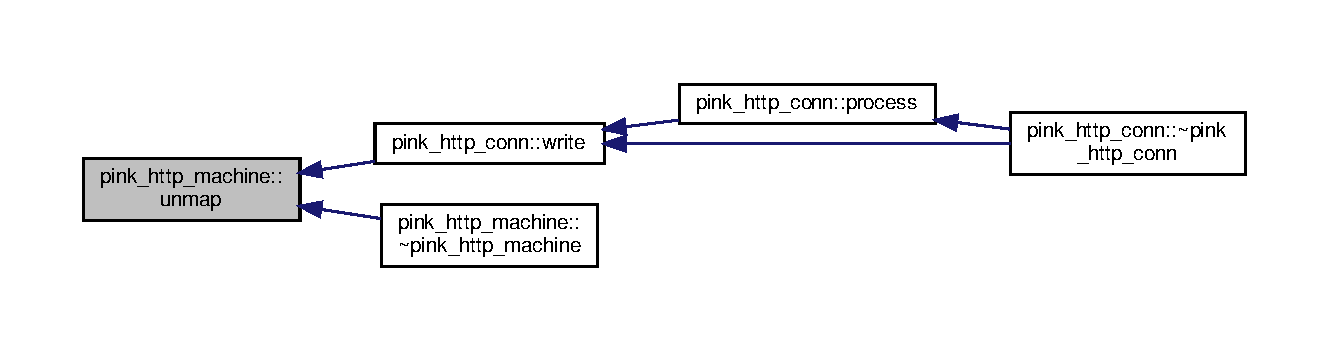
\includegraphics[width=350pt]{classpink__http__machine_a26debab8c361df5c79966f11e2b2dd17_icgraph}
\end{center}
\end{figure}


\subsection{Member Data Documentation}
\mbox{\Hypertarget{classpink__http__machine_a33993ee83910b37ae5672c6e6c94cac3}\label{classpink__http__machine_a33993ee83910b37ae5672c6e6c94cac3}} 
\index{pink\+\_\+http\+\_\+machine@{pink\+\_\+http\+\_\+machine}!F\+I\+L\+E\+N\+A\+M\+E\+\_\+\+L\+EN@{F\+I\+L\+E\+N\+A\+M\+E\+\_\+\+L\+EN}}
\index{F\+I\+L\+E\+N\+A\+M\+E\+\_\+\+L\+EN@{F\+I\+L\+E\+N\+A\+M\+E\+\_\+\+L\+EN}!pink\+\_\+http\+\_\+machine@{pink\+\_\+http\+\_\+machine}}
\subsubsection{\texorpdfstring{F\+I\+L\+E\+N\+A\+M\+E\+\_\+\+L\+EN}{FILENAME\_LEN}}
{\footnotesize\ttfamily constexpr int pink\+\_\+http\+\_\+machine\+::\+F\+I\+L\+E\+N\+A\+M\+E\+\_\+\+L\+EN = 1024\hspace{0.3cm}{\ttfamily [static]}}



Definition at line 87 of file pink\+\_\+http\+\_\+machine.\+h.

\mbox{\Hypertarget{classpink__http__machine_a4373363c5bd675e182f502d300157aa9}\label{classpink__http__machine_a4373363c5bd675e182f502d300157aa9}} 
\index{pink\+\_\+http\+\_\+machine@{pink\+\_\+http\+\_\+machine}!mime\+\_\+type@{mime\+\_\+type}}
\index{mime\+\_\+type@{mime\+\_\+type}!pink\+\_\+http\+\_\+machine@{pink\+\_\+http\+\_\+machine}}
\subsubsection{\texorpdfstring{mime\+\_\+type}{mime\_type}}
{\footnotesize\ttfamily std\+::unordered\+\_\+map$<$ string, string $>$ pink\+\_\+http\+\_\+machine\+::mime\+\_\+type\hspace{0.3cm}{\ttfamily [static]}}

{\bfseries Initial value\+:}
\begin{DoxyCode}
= 
                                \hyperlink{classpink__http__machine_ad6d404392628f4b2c94a4b30fefb62f8}{pink\_http\_machine::mime\_map\_init}()
\end{DoxyCode}


Definition at line 89 of file pink\+\_\+http\+\_\+machine.\+h.



The documentation for this class was generated from the following files\+:\begin{DoxyCompactItemize}
\item 
\hyperlink{pink__http__machine_8h}{pink\+\_\+http\+\_\+machine.\+h}\item 
\hyperlink{pink__http__machine_8cpp}{pink\+\_\+http\+\_\+machine.\+cpp}\end{DoxyCompactItemize}

\hypertarget{classpink__threadpool}{}\section{pink\+\_\+threadpool$<$ T $>$ Class Template Reference}
\label{classpink__threadpool}\index{pink\+\_\+threadpool$<$ T $>$@{pink\+\_\+threadpool$<$ T $>$}}
\subsection*{Public Member Functions}
\begin{DoxyCompactItemize}
\item 
\mbox{\Hypertarget{classpink__threadpool_a75dcfa67e83f32078d65f263cae5b118}\label{classpink__threadpool_a75dcfa67e83f32078d65f263cae5b118}} 
{\bfseries pink\+\_\+threadpool} (int thread\+\_\+number=8, int max\+\_\+requests=100000)
\item 
\mbox{\Hypertarget{classpink__threadpool_ae4bead5c98203b97c3caeae43296d295}\label{classpink__threadpool_ae4bead5c98203b97c3caeae43296d295}} 
bool {\bfseries append} (T $\ast$request, int flag)
\end{DoxyCompactItemize}


The documentation for this class was generated from the following file\+:\begin{DoxyCompactItemize}
\item 
pink\+\_\+thread\+\_\+pool.\+h\end{DoxyCompactItemize}

\hypertarget{classpink__time__heap}{}\section{pink\+\_\+time\+\_\+heap Class Reference}
\label{classpink__time__heap}\index{pink\+\_\+time\+\_\+heap@{pink\+\_\+time\+\_\+heap}}


{\ttfamily \#include $<$pink\+\_\+epoll.\+h$>$}

\subsection*{Public Member Functions}
\begin{DoxyCompactItemize}
\item 
\hyperlink{classpink__time__heap_a72c02a943378fc5573ba55c614fc4b8d}{pink\+\_\+time\+\_\+heap} ()=default
\item 
\hyperlink{classpink__time__heap_a45279534f708648c2f51d166fe0a376a}{pink\+\_\+time\+\_\+heap} (int init\+\_\+cap=1024)
\item 
\hyperlink{classpink__time__heap_a6aed9951c6c206e7752fa304d8fec612}{$\sim$pink\+\_\+time\+\_\+heap} ()
\item 
void \hyperlink{classpink__time__heap_aa74cc12fe4a94acbe75b70a3962a862f}{push} (\hyperlink{classconn__timer}{conn\+\_\+timer} $\ast$t)
\item 
void \hyperlink{classpink__time__heap_a331d1f993efc7bd50f8e6d10e5f1c6ee}{cancel} (\hyperlink{classconn__timer}{conn\+\_\+timer} $\ast$t)
\item 
\hyperlink{classconn__timer}{conn\+\_\+timer} $\ast$ \hyperlink{classpink__time__heap_ac0932b13390241373290a321ecf16600}{top} () const
\item 
void \hyperlink{classpink__time__heap_a5642ee3340cdee7983ed63770e7109d1}{pop} ()
\item 
void \hyperlink{classpink__time__heap_a9193dc948c6bb00005bf6639f2169b57}{tick} ()
\item 
bool \hyperlink{classpink__time__heap_ade64cf32193747380cb57c5709e28383}{empty} () const
\end{DoxyCompactItemize}


\subsection{Detailed Description}


Definition at line 24 of file pink\+\_\+epoll.\+h.



\subsection{Constructor \& Destructor Documentation}
\mbox{\Hypertarget{classpink__time__heap_a72c02a943378fc5573ba55c614fc4b8d}\label{classpink__time__heap_a72c02a943378fc5573ba55c614fc4b8d}} 
\index{pink\+\_\+time\+\_\+heap@{pink\+\_\+time\+\_\+heap}!pink\+\_\+time\+\_\+heap@{pink\+\_\+time\+\_\+heap}}
\index{pink\+\_\+time\+\_\+heap@{pink\+\_\+time\+\_\+heap}!pink\+\_\+time\+\_\+heap@{pink\+\_\+time\+\_\+heap}}
\subsubsection{\texorpdfstring{pink\+\_\+time\+\_\+heap()}{pink\_time\_heap()}\hspace{0.1cm}{\footnotesize\ttfamily [1/2]}}
{\footnotesize\ttfamily pink\+\_\+time\+\_\+heap\+::pink\+\_\+time\+\_\+heap (\begin{DoxyParamCaption}{ }\end{DoxyParamCaption})\hspace{0.3cm}{\ttfamily [default]}}

\mbox{\Hypertarget{classpink__time__heap_a45279534f708648c2f51d166fe0a376a}\label{classpink__time__heap_a45279534f708648c2f51d166fe0a376a}} 
\index{pink\+\_\+time\+\_\+heap@{pink\+\_\+time\+\_\+heap}!pink\+\_\+time\+\_\+heap@{pink\+\_\+time\+\_\+heap}}
\index{pink\+\_\+time\+\_\+heap@{pink\+\_\+time\+\_\+heap}!pink\+\_\+time\+\_\+heap@{pink\+\_\+time\+\_\+heap}}
\subsubsection{\texorpdfstring{pink\+\_\+time\+\_\+heap()}{pink\_time\_heap()}\hspace{0.1cm}{\footnotesize\ttfamily [2/2]}}
{\footnotesize\ttfamily pink\+\_\+time\+\_\+heap\+::pink\+\_\+time\+\_\+heap (\begin{DoxyParamCaption}\item[{int}]{init\+\_\+cap = {\ttfamily 1024} }\end{DoxyParamCaption})}



Definition at line 192 of file pink\+\_\+epoll.\+cpp.

\mbox{\Hypertarget{classpink__time__heap_a6aed9951c6c206e7752fa304d8fec612}\label{classpink__time__heap_a6aed9951c6c206e7752fa304d8fec612}} 
\index{pink\+\_\+time\+\_\+heap@{pink\+\_\+time\+\_\+heap}!````~pink\+\_\+time\+\_\+heap@{$\sim$pink\+\_\+time\+\_\+heap}}
\index{````~pink\+\_\+time\+\_\+heap@{$\sim$pink\+\_\+time\+\_\+heap}!pink\+\_\+time\+\_\+heap@{pink\+\_\+time\+\_\+heap}}
\subsubsection{\texorpdfstring{$\sim$pink\+\_\+time\+\_\+heap()}{~pink\_time\_heap()}}
{\footnotesize\ttfamily pink\+\_\+time\+\_\+heap\+::$\sim$pink\+\_\+time\+\_\+heap (\begin{DoxyParamCaption}{ }\end{DoxyParamCaption})}



Definition at line 202 of file pink\+\_\+epoll.\+cpp.



\subsection{Member Function Documentation}
\mbox{\Hypertarget{classpink__time__heap_a331d1f993efc7bd50f8e6d10e5f1c6ee}\label{classpink__time__heap_a331d1f993efc7bd50f8e6d10e5f1c6ee}} 
\index{pink\+\_\+time\+\_\+heap@{pink\+\_\+time\+\_\+heap}!cancel@{cancel}}
\index{cancel@{cancel}!pink\+\_\+time\+\_\+heap@{pink\+\_\+time\+\_\+heap}}
\subsubsection{\texorpdfstring{cancel()}{cancel()}}
{\footnotesize\ttfamily void pink\+\_\+time\+\_\+heap\+::cancel (\begin{DoxyParamCaption}\item[{\hyperlink{classconn__timer}{conn\+\_\+timer} $\ast$}]{t }\end{DoxyParamCaption})}



Definition at line 222 of file pink\+\_\+epoll.\+cpp.

Here is the call graph for this function\+:\nopagebreak
\begin{figure}[H]
\begin{center}
\leavevmode
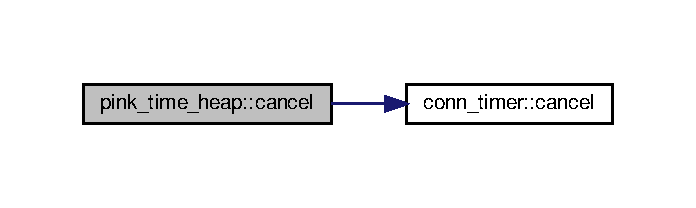
\includegraphics[width=334pt]{classpink__time__heap_a331d1f993efc7bd50f8e6d10e5f1c6ee_cgraph}
\end{center}
\end{figure}
\mbox{\Hypertarget{classpink__time__heap_ade64cf32193747380cb57c5709e28383}\label{classpink__time__heap_ade64cf32193747380cb57c5709e28383}} 
\index{pink\+\_\+time\+\_\+heap@{pink\+\_\+time\+\_\+heap}!empty@{empty}}
\index{empty@{empty}!pink\+\_\+time\+\_\+heap@{pink\+\_\+time\+\_\+heap}}
\subsubsection{\texorpdfstring{empty()}{empty()}}
{\footnotesize\ttfamily bool pink\+\_\+time\+\_\+heap\+::empty (\begin{DoxyParamCaption}{ }\end{DoxyParamCaption}) const}



Definition at line 258 of file pink\+\_\+epoll.\+cpp.

Here is the caller graph for this function\+:\nopagebreak
\begin{figure}[H]
\begin{center}
\leavevmode
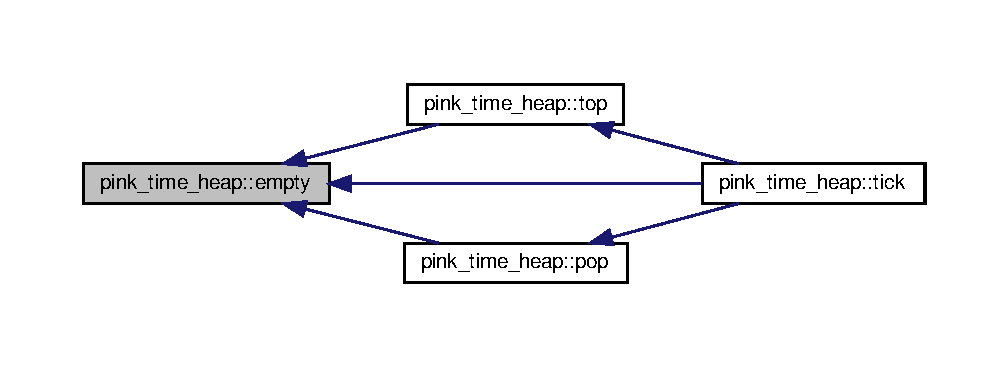
\includegraphics[width=350pt]{classpink__time__heap_ade64cf32193747380cb57c5709e28383_icgraph}
\end{center}
\end{figure}
\mbox{\Hypertarget{classpink__time__heap_a5642ee3340cdee7983ed63770e7109d1}\label{classpink__time__heap_a5642ee3340cdee7983ed63770e7109d1}} 
\index{pink\+\_\+time\+\_\+heap@{pink\+\_\+time\+\_\+heap}!pop@{pop}}
\index{pop@{pop}!pink\+\_\+time\+\_\+heap@{pink\+\_\+time\+\_\+heap}}
\subsubsection{\texorpdfstring{pop()}{pop()}}
{\footnotesize\ttfamily void pink\+\_\+time\+\_\+heap\+::pop (\begin{DoxyParamCaption}{ }\end{DoxyParamCaption})}



Definition at line 235 of file pink\+\_\+epoll.\+cpp.

Here is the call graph for this function\+:\nopagebreak
\begin{figure}[H]
\begin{center}
\leavevmode
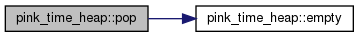
\includegraphics[width=341pt]{classpink__time__heap_a5642ee3340cdee7983ed63770e7109d1_cgraph}
\end{center}
\end{figure}
Here is the caller graph for this function\+:\nopagebreak
\begin{figure}[H]
\begin{center}
\leavevmode
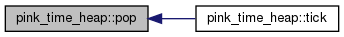
\includegraphics[width=330pt]{classpink__time__heap_a5642ee3340cdee7983ed63770e7109d1_icgraph}
\end{center}
\end{figure}
\mbox{\Hypertarget{classpink__time__heap_aa74cc12fe4a94acbe75b70a3962a862f}\label{classpink__time__heap_aa74cc12fe4a94acbe75b70a3962a862f}} 
\index{pink\+\_\+time\+\_\+heap@{pink\+\_\+time\+\_\+heap}!push@{push}}
\index{push@{push}!pink\+\_\+time\+\_\+heap@{pink\+\_\+time\+\_\+heap}}
\subsubsection{\texorpdfstring{push()}{push()}}
{\footnotesize\ttfamily void pink\+\_\+time\+\_\+heap\+::push (\begin{DoxyParamCaption}\item[{\hyperlink{classconn__timer}{conn\+\_\+timer} $\ast$}]{t }\end{DoxyParamCaption})}



Definition at line 207 of file pink\+\_\+epoll.\+cpp.

\mbox{\Hypertarget{classpink__time__heap_a9193dc948c6bb00005bf6639f2169b57}\label{classpink__time__heap_a9193dc948c6bb00005bf6639f2169b57}} 
\index{pink\+\_\+time\+\_\+heap@{pink\+\_\+time\+\_\+heap}!tick@{tick}}
\index{tick@{tick}!pink\+\_\+time\+\_\+heap@{pink\+\_\+time\+\_\+heap}}
\subsubsection{\texorpdfstring{tick()}{tick()}}
{\footnotesize\ttfamily void pink\+\_\+time\+\_\+heap\+::tick (\begin{DoxyParamCaption}{ }\end{DoxyParamCaption})}



Definition at line 245 of file pink\+\_\+epoll.\+cpp.

Here is the call graph for this function\+:\nopagebreak
\begin{figure}[H]
\begin{center}
\leavevmode
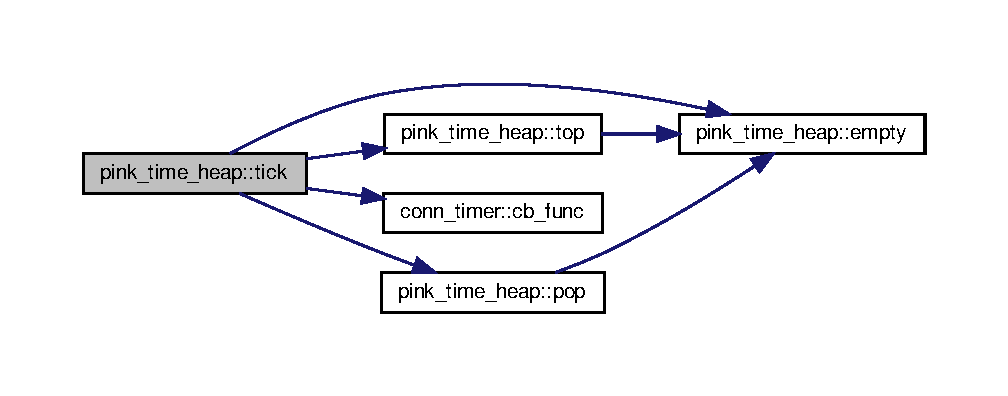
\includegraphics[width=350pt]{classpink__time__heap_a9193dc948c6bb00005bf6639f2169b57_cgraph}
\end{center}
\end{figure}
\mbox{\Hypertarget{classpink__time__heap_ac0932b13390241373290a321ecf16600}\label{classpink__time__heap_ac0932b13390241373290a321ecf16600}} 
\index{pink\+\_\+time\+\_\+heap@{pink\+\_\+time\+\_\+heap}!top@{top}}
\index{top@{top}!pink\+\_\+time\+\_\+heap@{pink\+\_\+time\+\_\+heap}}
\subsubsection{\texorpdfstring{top()}{top()}}
{\footnotesize\ttfamily \hyperlink{classconn__timer}{conn\+\_\+timer} $\ast$ pink\+\_\+time\+\_\+heap\+::top (\begin{DoxyParamCaption}{ }\end{DoxyParamCaption}) const}



Definition at line 229 of file pink\+\_\+epoll.\+cpp.

Here is the call graph for this function\+:\nopagebreak
\begin{figure}[H]
\begin{center}
\leavevmode
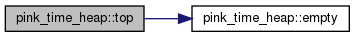
\includegraphics[width=338pt]{classpink__time__heap_ac0932b13390241373290a321ecf16600_cgraph}
\end{center}
\end{figure}
Here is the caller graph for this function\+:\nopagebreak
\begin{figure}[H]
\begin{center}
\leavevmode
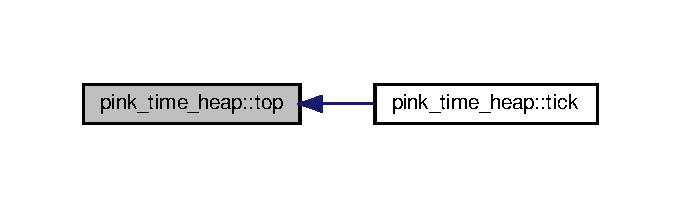
\includegraphics[width=327pt]{classpink__time__heap_ac0932b13390241373290a321ecf16600_icgraph}
\end{center}
\end{figure}


The documentation for this class was generated from the following files\+:\begin{DoxyCompactItemize}
\item 
\hyperlink{pink__epoll_8h}{pink\+\_\+epoll.\+h}\item 
\hyperlink{pink__epoll_8cpp}{pink\+\_\+epoll.\+cpp}\end{DoxyCompactItemize}

%--- End generated contents ---

% Index
\backmatter
\newpage
\phantomsection
\clearemptydoublepage
\addcontentsline{toc}{chapter}{Index}
\printindex

\end{document}
